%%%%%%%%%%%%%%%%%%%%%%%%%%  ltexpprt.tex  %%%%%%%%%%%%%%%%%%%%%%%%%%%%%%%%
%
% This is ltexpprt.tex, an example file for use with the SIAM LaTeX2E
% Preprint Series macros. It is designed to provide double-column output. 
% Please take the time to read the following comments, as they document
% how to use these macros. This file can be composed and printed out for
% use as sample output.

% Any comments or questions regarding these macros should be directed to:
%
%                 Donna Witzleben
%                 SIAM
%                 3600 University City Science Center
%                 Philadelphia, PA 19104-2688
%                 USA
%                 Telephone: (215) 382-9800
%                 Fax: (215) 386-7999
%                 e-mail: witzleben@siam.org


% This file is to be used as an example for style only. It should not be read
% for content.

%%%%%%%%%%%%%%% PLEASE NOTE THE FOLLOWING STYLE RESTRICTIONS %%%%%%%%%%%%%%%

%%  1. There are no new tags.  Existing LaTeX tags have been formatted to match
%%     the Preprint series style.    
%%
%%  2. You must use \cite in the text to mark your reference citations and 
%%     \bibitem in the listing of references at the end of your chapter. See
%%     the examples in the following file. If you are using BibTeX, please
%%     supply the bst file with the manuscript file.
%% 
%%  3. This macro is set up for two levels of headings (\section and 
%%     \subsection). The macro will automatically number the headings for you.
%%
%%  5. No running heads are to be used for this volume.
%% 
%%  6. Theorems, Lemmas, Definitions, etc. are to be double numbered, 
%%     indicating the section and the occurence of that element
%%     within that section. (For example, the first theorem in the second
%%     section would be numbered 2.1. The macro will 
%%     automatically do the numbering for you.
%%
%%  7. Figures, equations, and tables must be single-numbered. 
%%     Use existing LaTeX tags for these elements.
%%     Numbering will be done automatically.
%%   
%%
%%%%%%%%%%%%%%%%%%%%%%%%%%%%%%%%%%%%%%%%%%%%%%%%%%%%%%%%%%%%%%%%%%%%%%%%%%%%%%%



%\documentclass[twoside,leqno,twocolumn]{article}  
\documentclass[12pt]{article}
\usepackage{sbc-template} 
\usepackage{makeidx}
\usepackage{subfigure}
\usepackage{multirow}
\usepackage{color}
\usepackage{times}
\usepackage{graphicx,url}
\usepackage{rotating}
\usepackage{amssymb}
\usepackage{epsfig}
\usepackage[section]{algorithm}
\usepackage{algorithmicx}
\usepackage[noend]{algpseudocode}
\usepackage{multirow}
\usepackage[utf8]{inputenc}
\usepackage{colortbl}
\usepackage{booktabs}
%\usepackage{graphicx}
\usepackage{rotating}
\usepackage{epstopdf}

\sloppy

\title{Building Semantic Profiles of Social Network User Groups}
\author{Aluno: Paulo Viana Bicalho \inst{1}, Orientadora: Gisele Lobo Pappa \inst{1} }

\address{Universidade Federal de Minas Gerais  (UFMG)\\ }

\begin{document}

\newcommand{\fhmourao}[1]{{\color{red}[#1]}}
\newcommand{\gi}[1]{{\color{blue}[#1]}}
\newcommand{\method}{UPsCAle }

%\setlength{\abovecaptionskip}{0.2pt}
%\setlength{\belowcaptionskip}{0.2pt}
%\setlength{\abovedisplayskip}{0pt}
%\setlength{\belowdisplayskip}{0pt}

%\linespread{0.5}

%\setcounter{chapter}{2} % If you are doing your chapter as chapter one,
%\setcounter{section}{3} % comment these two lines out.

%\title{\Large{Building Semantic Profiles of Social Network User Groups}}
%\author{Tiago Cunha\thanks{Federal University of Minas Gerais.} 
%\and 
%Fernando Mour\~ao \footnotemark[1]
%\and 
%Paulo Bicalho \footnotemark[1]
%\and 
%Gisele L. Pappa \footnotemark[1]
%\and 
%Wagner Meira Jr. \footnotemark[1]\\
%}









\date{}

\maketitle

 
%\pagenumbering{arabic}
%\setcounter{page}{1}%Leave this line commented out.

\begin{abstract} \small\baselineskip=9pt 
Information about users in social networks is highly valuable for
understanding user preferences regarding products, brands or politics. Many
works have tried to cluster or classify each user according to her common
interests. This paper, in contrast, proposes an approach to characterize
groups of users with a common interest, expressed through relationships in
social networks. In the characterization process, users preferences are
defined by the semantic topics they most discuss. In order to find semantic
topics, we propose a method that successfully merges topics found through
matrix factorization by performing random walks in a latent-topic transition
graph. Experiments were performed in documents datasets for easier evaluation
and in social network datasets. The method showed to be scalable and accurate
in identifying the semantic topics inside a selected group of users.\\
\textbf{Keywords: users profiles, topic discovery, NMF}
\end{abstract}

 

\section{Introduction}

Twitter has already proven to be a powerful source of information for  monitoring
trends, sentiments and topics, 
%\cite{ramage2010characterizing}, 
but to
this date not a lot is known about Twitter users.  The majority of studies
regarding users focuses on issues such as the demographics of Twitter, 
%(including methods for inferring sex, age or location information)
%\cite{davisjr:2011}, 
community detection %\cite{java2007we} 
and measures to assess user influence.  However, only a 
few works have focused on another very interesting issue: user profiling\cite{abel:2011}. 

A user profile may contain different elements, including user preferences (as
expressed in messages), personal information (such as gender and location) or
social network behavior (usage time and number of posts per day, among others).
In this work we define users' profiles based on their general preferences,
where a preference is defined by a \textit{semantic topic} discussed in their
posts. 
 
In contrast with previous methods for creating user profiles for specific user
accounts \cite{pennacchiotti2011democrats,abel2011semantic}, here we are
interested in generating profiles of \textit{groups of users}.  These groups
comprise users that share at least one common interest, which may become
explicit when they follow the same Twitter account or frequently discuss the
same topic. Identifying such groups and profiles is of great value for
companies, which can take advantage of them for targeted marketing,
recommendation, or to better understand users preferences over time. 

By profiling groups of users we avoid problems of privacy and data scarcity
while being able to determine the underlying habits and preferences
\cite{zheleva:2009}.  On the other hand, there are several challenges in
such profiling task. The first challenge arises when determining the
semantic topics that characterize the users, since they must be,
simultaneously, the \textit{smallest representative} set of \textit{highly
cohesive} and \textit{non-fragmented} topics observed in a set of messages.
The second challenge is related to the efficiency of the profiling method,
since the number of posts is usually huge and increasing. The third challenge
is the lack of context associated with microblog messages such as Twitter,
making the topic detection, and thus profiling particularly challenging.
The fourth challenge is, given a set of semantic topics, to identify the 
users that will compose each group, coupling with their diversity
and the complexity of the topic. Finally, we may summarize the profile of
each group based on the semantic topics that arise in the group and 
their intensity.

Formally, considering that we extract semantic topics from users posts, any set
of users $U$ can be characterized by a weighted set of preferences
$<$$p_1$,$p_2$,$\ldots$,$p_n$$>$, where $p_x$ represents a semantic topic
identified from the posts of the group. Although we focus just on topics as
preferences in this work, other personal user characteristics may be added to
the preference set later.

In order to build semantic profiles of groups of users, we propose the UPsCAle
(User Profile CreAtor) framework, which is organized in three main phases: (i)
it identifies semantic sub-topics of a user group using a traditional matrix
factorization method; (ii) it merges semantic sub-topics into more cohesive and
unique semantic topics; (iii) it maps the final set of semantic topics into
users profiles.  In the first phase, we benefit from the fact that the task has
been extensively studied~\cite{pons2007topic}, and employ a Non-negative Matrix
Factorization (NMF) \cite{berry2007algorithms}, which is capable of generating
good-quality topics, despite vocabulary overlaps.  However, these semantic
topics may still lack cohesion\cite{cheng:2013}, and we propose a new method
for phase (ii), based on Markovian theory, for merging topics in order to
generate more cohesive topics.  Finally, the desired profiles are then
generated based on a simple strategy that has shown to perform surprisingly
well.

In summary, this paper has two main contributions. The first, a new generic
semantic topic identification method that can be used in any topic detection
task and optimizes the three contradictory but desirable properties in topic
identification simultaneously: representativeness, cohesion and
non-fragmentation. The method is also scalable, efficient and handles the lack
of context usually inherent to microblogs and other social media platforms.
The second contribution is a simple yet effective method to define users
profiles considering groups of users, represented by a weighted set of
preferences that initially correspond to semantic topics. 

\method was evaluated in two phases. First, we tested the topic identification
method in both text and social network collections where the main topics were
known. Second, we performed a case study with over 50,000 users that are
Twitter followers of Barack Obama, considering more than the 700,000 messages
posted during the American Elections in 2012. The results showed that the
method is able to generate less fragmented and more concise topics when
compared to other state of the art methods.% for topics identification.
Such topics enabled the determination of good quality profiles, as the results
show.

%WMJ: do we have anything to say about users?

%The remainder of this paper is organized as follows. Section 2 discusses related work in both user profiles and semantic topic identification. Section 3 introduces UPscALe, the framework developed to find users profiles according to semantic topics. Section 4 describes the experimental methodology, where tests wih both labeled and unlabeled data are performed. Finally, Section 5 draws conclusions and discusses future work directions.


\section{Related Work}\label{sec:related}

%Understanding user behaviors in social networks have become a primary goal of several researches recently \cite{}. Indeed, understanding how users behave, interact and discuss reveals useful information for various scientific and commercial  applications, such as recommendation of services or information, modeling of community formation and modeling of information  propagation \cite{. Thus, a growing number of efforts aim to identify groups of Social Media users with common  interests, expressed by textual data published in the Social Media. Proposals for this task range from traditional clustering algorithms applied to textual data \cite{ to Natural Language Process (NLP) based methods \cite{chen1995topic}.

%Differently, this work aims to characterize the interests related to each group of users previously identified in a domain, as  well as providing meaningful descriptions for these interests. Specifically, we consider as `interest' a semantic topic recurrently  discussed in a set of posts published by members of a specific group of users. Also, we consider that such groups of users were  previsously defined, for example, by some attribute inherent to users or by any existing proposal for identifying group of users  applied to Social Media content. An immediate question in this case is: why does our goal differ from the identification of group  of users, since the definition of these groups is usually based on modeling common interests? A first problem is that several of the  techniques used for grouping users do not concern to provide semantic topics interpretable by humans \cite{ayad2002topic,li2003topic}.  Thus, often the goal is to generate a model able to identify dependencies that allow the definition of groups. However, these  dependencies may not explain the interests related to each group. Second, even the few studies focused in describing semantic  topics exhibit two main limitations. Current works focus on defining the semantic topics defined by a single user \cite{abel2011semantic}.  It differs significantly from group analyses since different users express interest on a same topic through different vocabularies.  Hence, considering them individually and summarizing individual results may not cover some common interests. Further, these works  are based on a poor definition of what represents a `semantic groups`. As aforementioned, we assume that a tangible definition of `semantic' requires three requirements: coehsion, representativity and fragmentation. Most of the existing proposal take into account only of of these requirements, providing incomplete, redundant or not well defined semantic topics.
%A variety of works for characterizing user behavior in social media were proposed in the past years \cite{kaplan2010users,Benevenuto2009}. However, the great majority of methods focused on users wants to classify them according to a set of predefined categories, such as political view , or according to other personal information, such as location, age, among others \cite{pennacchiotti2011democrats}.

This section reviews methods for both semantic
topic identification and user profiling.
%and discuss how they compare to the method proposed here.
%In the second part we analyze methods for user profiling.
Concerning topic identification, there are four main efforts in the literature: (i) clustering, which includes traditional data mining algorithms applied to textual data \cite{aggarwal2012mining}; (ii) natural-language processing (NLP) methods, well-known as the most effective for semantic analysis in several scenarios \cite{mihalcea2011graph} but also the ones that require most effort to define properly the semantic representation in each domain; (iii) probabilistic, such as Latent Dirichlet Allocation (LDA), which employ a similar interpretation to data as linear algebra methods and (iv) non-probabilistic, which are the methods we are interested in.


%The first group of efforts comprises traditional clustering algorithms that explore data correlations in order to identify distinct groups of topics. %\cite{ozmutlu2006automatic}. This group includes traditional data mining algorithms applied to textual data \cite{aggarwal2012mining}.%,pons2007topic}.  
%The major problem with this approach
%is that the data correlations consider the existence of recurring and directly observable patterns in the dataset. This is usually not the case in textual data, since one concept can be described in many ways. 

Non-probabilistic methods, such as matrix
factorization and sparse coding
\cite{bai:2013,cheng:2013}, assume that there are few latent factors not directly observable from
data that are able to represent most of the original data.  In this case,
each latent factor is defined as a semantic topic. 
%, as they are derived from co-occurrences among sets of items.  
As one may refer to the same semantic topic using different vocabularies, we say this type of technique actually generates fragmented or even redundant representations
of semantic topics, known as semantic sub-topics. 

In order to deal with the problem of redundancy, Kuhn et al.
\cite{kuhn2007semantic} uses a Latent Semantic Indexing (LSI) method followed
by a clustering process to identify semantic topics from the source codes of a
system. 
%Their idea was to better explain the general components of the code. 
Their method identifies latent factors in the raw data, and then represents
the original files using the new N-dimensional space defined by the $N$ latent
factors. Next, it clusters the files using a co-variance matrix  represented
on the top of this new space of files. 
%The work proposed here goes into this direction.  
The main drawback of this approach is the use of co-variance
matrices, which do not scale to large volumes of data.

%ADDED
For short texts such as tweets, matrix factorization methods also have problems dealing with highly sparse data, a problem attacked in \cite{cheng:2013}. Here we minimize this problem by using a set of tweets instead of a single one. 

%The third group refers to probabilistic methods, such as Latent Dirichlet Allocation (LDA), which
%employ a similar interpretation to data as linear algebra methods. However,
%they use a statistical framework of analysis, ensuring a better modeling of
%uncertain data \cite{ramage2010characterizing}.  Their main drawback
%of is in the complexity for identifying appropriate models and
%parameters that identify semantic topics correctly.

%, which has been shown as a practical challenge. 

%Finally, the fourth group includes techniques derived from NLP. They are well-known as the most effective methods for semantic analysis in several scenarios \cite{mihalcea2011graph}. However, these methods are also the most expensive, requiring a significant human effort to define properly the semantic representation in each domain \cite{liu2004conceptnet}.Hence, applying this type of methods in environments characterized by dynamicity and huge volumes of data as social media is not appropriate.

%WMJ: this last argument is quite weak

Regarding user profiling methods, they can build user profiles from different
user characteristics, which include user preferences (found in messages),
personal information (such as gender and location) or social network behavior
(usage time, number of posts per day, among others)
\cite{tao:2011,pennacchiotti2011democrats}.  Previous works have
already used the text from tweets to help classifying users, and even applied
linear algebra methods, such as LDA, in order to find topics that are not
explicitly mentioned in the text. Pennacchiotti et al.
\cite{pennacchiotti2011democrats}, for instance, proposes an architecture that
builds user profiles in order to classify Twitter users with regards to
particular political views (e.g., Democrats vs.  Republicans).  The authors use
features such as the linguistic content of the tweets posted by a specific user
and his/her social behavior. The information extracted is given to a machine
learning algorithm that classifies users as republicans or democrats.  A
description of interests related to each class is also provided by an LDA-based
method. However, the main problem in this case is that the authors assume the
existence of training data, which is not always available for semantic
analysis. 

Tao et al. \cite{tao:2011} and Abel et al. \cite{abel2011semantic}, in
contrast, use tweets to infer user interest profiles. Here, instead of
identifying general topics, the authors first enrich the tweets by identifying
and extracting a set of 39 pre-defined entities using
OpenCalais\footnote{www.opencalais.com}, and also consider hashtags.
\cite{tao:2011} also uses a set of 19 predefined topics to identify the users
preferences. The identified preferences are weighted and shown with clould tags
and graphs. In \cite{abel2011semantic}, in turn, as the final goal of the
authors is to use the profiles to improve news recommendation, the authors also
identify links in tweets and associate them with the original webpages, which in
most cases refer to news. Topics are then extracted from these identified news
also using the OpenCalais taxonomy. The authors compared profiles built with
different combinations of the information described above, and concluded that
entity-based and topic-based profiles make the semantics of the preferences
much more explicit than other types of information.

From the methods mentioned above, the works of \cite{kuhn2007semantic} and \cite{pennacchiotti2011democrats} are the most similar to ours.
However, in contrast with \cite{kuhn2007semantic}, \method represents a scalable and robust strategy for modeling semantic topics. It is also independent of training data, and does not require a set of predefined topics to work with.
%We do that by producing a hierarchical clustering of the latent factors generated by a NMF method based on a probabilistic transition graph among them.  





\section{\method: A Framework for Creating Users Profiles }

This section describes \method, the framework proposed to identify semantic
profiles for a set of targeted users from Twitter. As previously described,
the users profiles are a set of weighted preferences, representing a semantic
topic frequently discussed in their posts $D$.  Figure~\ref{frameworkFig}
illustrates the framework.  Steps one to four, i.e.,text
preprocessing, data modelling and extraction of latent factors, do not differ
from what has been done in the literature so far. The main contribution of the
framework is steps five to nine, where semantic sub-topics are merged into
semantic groups and then used to describe user preferences. Finally, these
user preferences are used to generate users semantic profiles.

The text preprocessing phase follows the traditional steps of text
preprocessing in information retrieval, which includes the removal of special
characters, stop-words, plural and genre
markers, and the conversion of verbs to infinitive.  After preprocessing, the
data modelling phase creates a matrix, given as input to a matrix
factorization method.

The data has three dimensions to be considered as part of the matrix: users,
terms and posts. Our final goal is to identify the topics most discussed by
the users in a given domain. Hence, one intuitive representation would be a
matrix of \textit{users} x \textit{terms}, once topics appear from
correlations between terms, and we want to associate topics with users.

However, the set of terms that represent a user will probably refer to more than one topic. As a post is usually made of one sentence expressing the user's opinion or preference in a specific matter, sets of posts will represent sets of topics. For this reason, data is represented as a matrix of \textit{posts} $\times$ \textit{terms}, making the correlation between different topics simpler to identify.
The term associated with each position in the matrix is represented using the term frequency (TF), which showed better results than a TF~X~IDF representation. 
%Although tests with TF~X~IDF were performed, tests with TF were performed better, as the definition of topic is a \emph{frequently mentioned} concept in a set of posts.

After these initial steps, the resulting matrix is used to identify latent factors or semantic sub-topics (representing relations between different terms) using a Non-negative Matrix Factorization (NMF) methods, which generates semantic topics that will be associated with user preferences. From the set of user preferences, users profiles are generated. These two steps are detailed in the next sections. 


\subsection{Identifying latent factors}
\label{primaryFactors}

As discussed in Section~\ref{sec:related}, 
many works in the literature have dealt with the problem of identifying latent factors. Here we work with NMF because it does not assume that latent factors compose
a space of independent variables. Further, NMF provides a more intuitive modelling of documents through these factors, defining each document
as a sum of positive components. We can briefly describe NMF as follows. Given an input matrix $A \in \mathbb{R}^{m \times n}$,
where each line represents a post and each column represents a term, and an integer  $k$ $<$ $min\{m, n\}$, representing the number of desired latent factors, NMF finds two non-negative matrices $W$ $\in$ $\mathbb{R}^{m \times k}$ and $H$ $\in$ $\mathbb{R}^{n \times k} $, where $A$ $\approx$ $W H^T$.

Defining $k$ for NMF is not simple, since it is widely
believed that NMF is a non-convex problem with a unique solution, and only local minima can be found \cite{lin2007convergence}. Here we propose a heuristic for finding $k$ based on the variability analysis of the post collection, as the objective of this phase is to identify as many distinct relevant topics as possible.

\begin{figure}[!t]
\centering
	\epsfig{file=figures/framework.eps,width= 3.2in,height=2.25in}
%	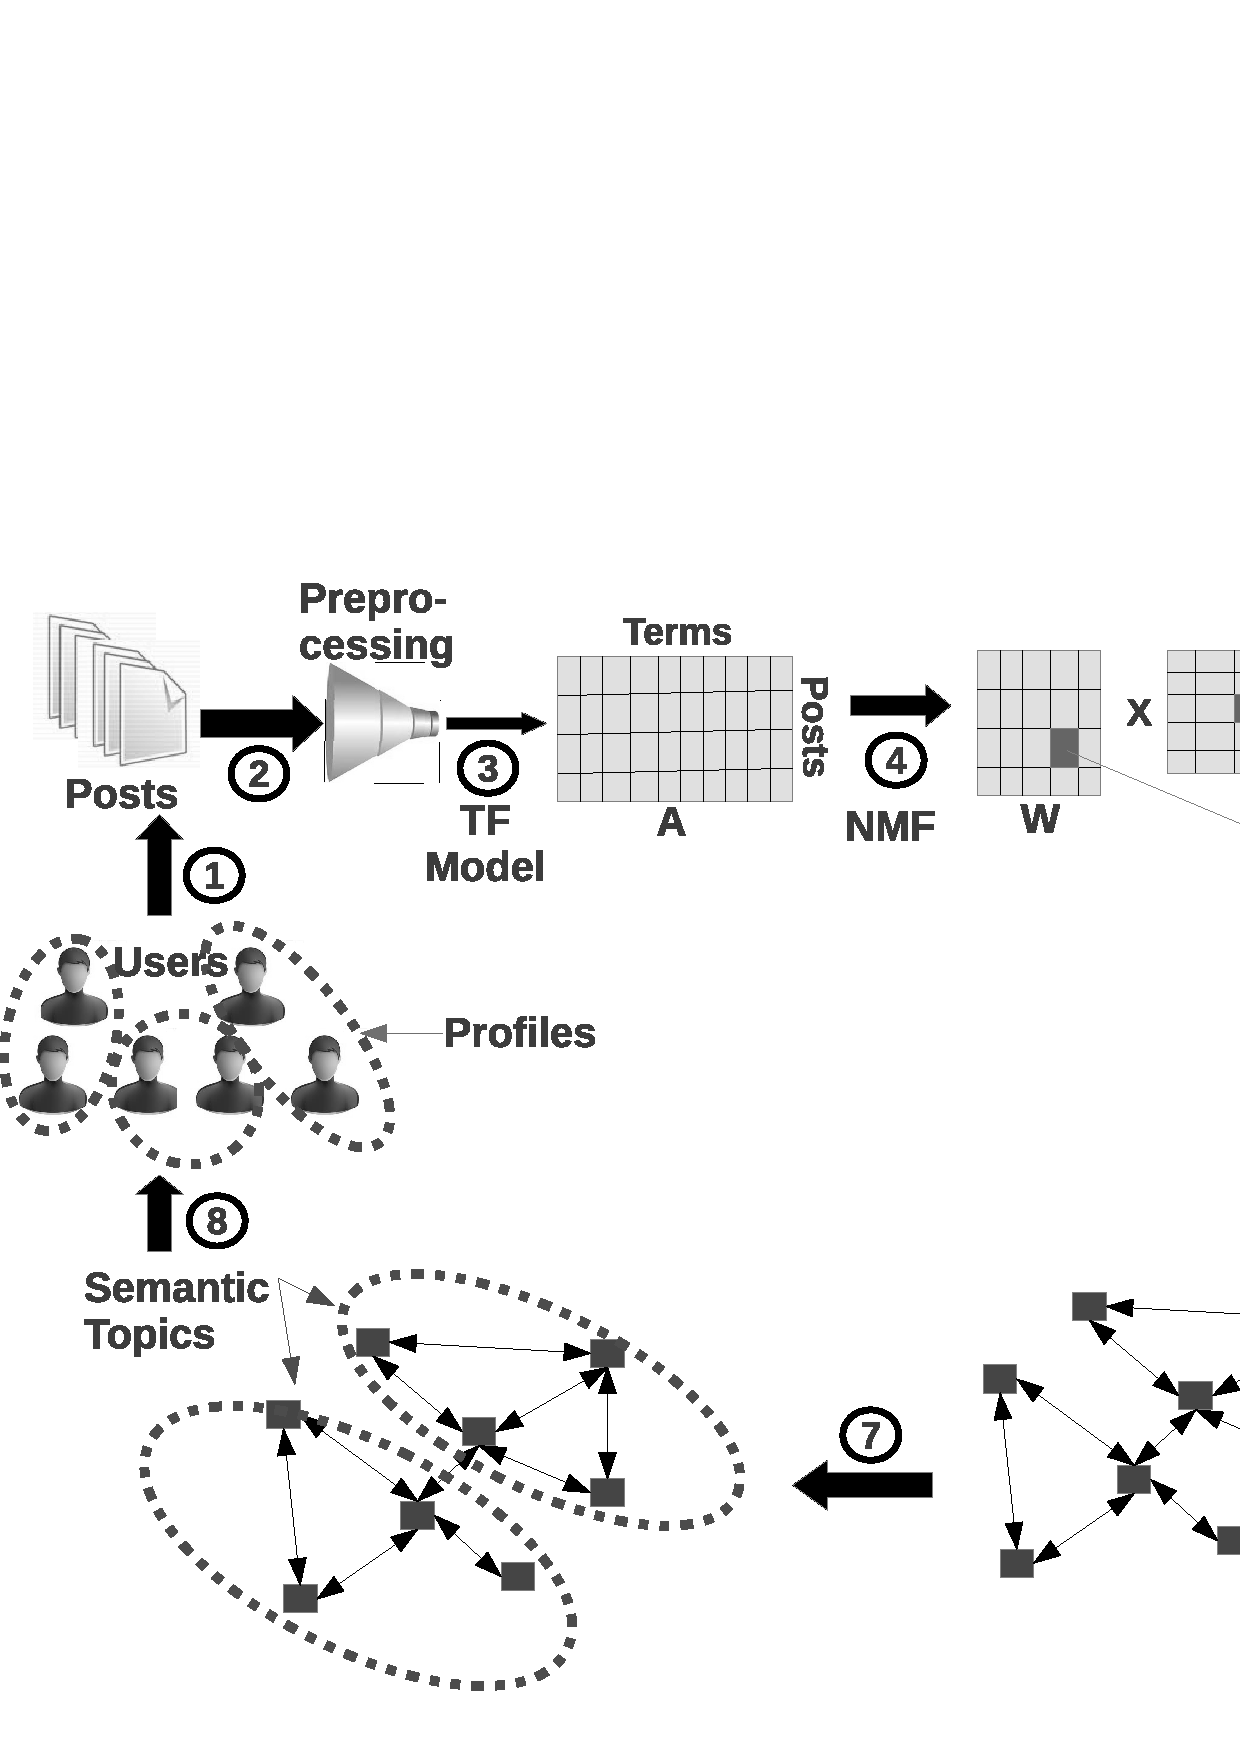
\includegraphics[width= 3.4in,height=2.45in]{figures/framework.pdf}
\vspace{-0.25cm}
\caption{\method: a framework for user semantic profile identification}
\label{frameworkFig}
\vspace{-0.25cm}
\end{figure}


% WMJ: premissa muito forte.
%We assume that the x\% most representative topics would define around x\% of the observed variability on each
%collection and vice-versa. 

We assume that the dimensions of highest variability define the most representative topics on each collection.
Thus, by knowing the number $k$ of topics necessary to provide x\% variability is enough to identify the number of most representative topics. In this sense, we run a Principal Component Analysis (PCA) method 
to estimate $k$. The rationale behind this choice is that the PCA is well-known for returning an ordered set of linearly
independent components that represent the dimensions of most variability on the data. According to the theory of Principal Component Analysis (PCA) \cite{johnson2002applied}, the total population variance (tpv) can be described as $\sum_{i=1}^{k} \lambda_{i}$, 
%\[
%\mbox{Total Populational Variance} = \sum_{i=1}^{k} \lambda_{i}
%\]
where $\lambda_{i}$ is the $i^{th}$ eigenvector of the co-variance matrix associated with the input matrix of posts $\times$ terms $A$ \cite{johnson2002applied}. 

The number $k$ of eigenvectors is chosen based on the desired $tpv$, or
equivalently to the percentage of desired representativeness. Hence, the framework replaces $k$ by a more intuitive parameter, which is the x\% most representative topics. 

%Again, it is important to emphasize that it is a heuristic, since NMF does not guarantee to find the $k$ dimensions of most variability. However, since matrix $W$ and $H$ found by NMF are non-orthonormal bases that minimize a $k\mbox{-}rank$ approximation to the original matrix $A$, in general its local minima solutions provide good approximations. However, bounds on the quality of NMF solutions is an open question in the literature \cite{berry2007algorithms}.

\subsection{Finding Semantic Topics}
\label{sec:merge}

We have already discussed that matrix factorization methods produce semantic
sub-topics, but they are not able to guarantee that the latent factors found
represent \textbf{distinct}, \textbf{representative} and \textbf{cohesive}
semantic topics. These three properties are important to show the topics are
as independent and disjunctive as possible.  According to these properties,
the semantic topic identification problem can be defined as: identify the
minimum number of semantic topics that represent, with high intern cohesion
and low fragmentation the most representative topics in a set of posts $D$.
Note that we are not interested in identifying all topics, but the most
representative subset.

The main objective of \method is to find topics with these three properties, which is a real challenge. Representativeness refers to the frequency of
the topics in D. However, it cannot be directly measured once different
vocabularies might refer to the same topic. These different vocabularies have
a direct impact on cohesion. Cohesion is defined as the capacity of a topic
being associated with a single subject. Finally, the topics have to be the
least fragmented as possible. This is necessary because topics are actually a
hierarchy of subtopics. For instance, when we talk about sports, we can talk
about football or tennis. In general, the existing techniques are able to
define each subtopic as a distinct topic, which generates a fragmented set of
topics about the same subject. This is one of the main differences from our
method to the others: identify non-fragmented semantic topics.

In order to merge semantic sub-topics, we first assume latent factors are modelled by a stochastic process, and that there is a
probability of reaching a factor $f'$ when leaving a factor $f$. Hence, we first represent the users, posts and terms as a tripartite graph, and transform it into a transition graph between different latent factors. We then perform a random walk between latent factors on this graph, and merge factors with high probabilities of mutually reaching each other.


\subsubsection{Creating a tripartite graph}

The NMF output matrices describe the relations between the latent factors found and the input terms and posts. The output $m \times k$ matrix $W$ represents the $m$ input posts through $k$ latent
factors. Each value $W_{ij}$ greater than zero defines both a directed edge
from post $p_i$ to latent factor $f_j$ and an edge in the opposite direction
from $f_j$ to $p_i$. Similarly, matrix $H$ of $n \times k$ dimensions
describes each term through $k$ factors, and each cell $H_{ij}$ greater than
zero defines a relation between a term and a latent factor.\looseness=-1

%\begin{figure}[!ht]
%\centering
%	\subfigure[]{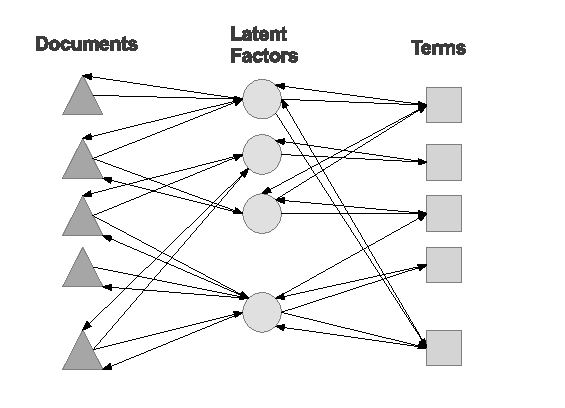
\epsfig{file=figures/tripartiteGraph.eps,width= 2.3in,height=1.45in}} \label{tripartiteGraph}
%	\hfill
%	\subfigure[]{}
%\epsfig{file=figures/tripartiteSemanticGraph.eps,width= 2.3in,height=1.45in}
%\vspace{-0.25cm}
%\caption{Example of a Tripartite Graph}\label{tripartiteGraph}
%\end{figure}

Based on this relation, we build a weighted directed tripartite graph $G_t$ with three types of nodes $T$, $F$ and $D$,
representing the terms, latent factors and posts, respectively.
%, as illustrated in Figure~\ref{tripartiteGraph}.
The intuition behind this graph is that a term can be associated with more than one latent factor (e.g., the term \textit{depression} might be present in the topic about health and politics with different meanings) as a post can talk about one or more latent factors (e.g., the same post can talk about sports and food ``Watching the football at Albanos while eating the best pesto spaghetti ever \#goPSG"). 
Each edge weight represents the intensity of the relationship between
two nodes, and the graph weights are given by the values of $W$ and $H$. As the values of the output matrices of
NMF are always positive, we used the normalized values of $W_{ij}$ and $H_{ij}$ as edge weights. Edges leaving a
term or post towards a latent factor, $W_{ij}$ or $H_{ij}$, are normalized by the sum of the values in the $i^{th}$
line of $W$ or $H$, making the sum of all leaving probabilities equals to $1$. Analogously, for edges leaving from
latent factors to terms/posts, we normalize their values by the sum of the values of the $j^{th}$ column.


\subsubsection{Building the Topic Transition Graph}

From the tripartite graph $G_t$, we want to convert it into a new graph $G$ describing only relationships between
latent factors in $F$. 
As the edge weights in $G$ are normalized, each weight can be interpreted
as a probability of leaving one node and reaching directly a different one. Following this rationale, each latent factor
$f_i \in F$ has also an indirect probability of reaching another factor $f_j \in F$ through terms and posts. We want to
transform these indirect links into direct relations between factors. 
Having a graph that represents only latent factors, we can then calculate the probabilities of a random walker leaving a  latent factor $f_i$ and reaching a latent factor $f_j$.
In order to do that, we transform this two-step probabilistic
paths into a single edge by using Equation~\ref{transitionEquation}. Note that we join these probabilities by summing up their results, but other kinds of combinations could be tested.

\begin{scriptsize}
\begin{equation} \small
P(f_i \!\rightarrow \!f_j)\! = \!\!\sum_{k \in T^{f_i}}\!\!\! P( t_k|f_i) \times P( f_j|t_k)  + \!\sum_{k \in D^{f_i}}\!\!\! P(d_k|f_i) \times P (f_j|d_k) \\
\label{transitionEquation}
\end{equation}
\end{scriptsize}
%P(f_i, f_j) = \sum_{k \in T^{f_i}} P(f_i, t_k) \times P(t_k, f_j) + \sum_{k \in D^{f_i}} P(f_i, d_k) \times P(d_k, f_j)

\noindent where $T^{f_i}$ and $D^{f_i}$ are the sets of terms and posts with an input edge $f_i$. In Equation~\ref{transitionEquation},
the first sum represents all indirect paths from $f_i$ to $f_j$ passing through the terms, while the second comprises the indirect paths through documents.

The resulting graph $G$ is represented by a stochastic transition matrix $M$,
i.e., where the sum of each row in $M$ is equal to 1. As we are concerned
with semantic relations among latent factors, and that not semantically
correlated topics may share a subset of terms, it is important to distinguish
effective relations from noisy ones. A noisy relation is defined as an edge in
$G_i$ with transition probability smaller than the random transition
probability in a graph of the same size. Noisy relations are identified and
removed from $G$ by setting to zero their corresponding cells in matrix $M$. In
order to ensure that $M$ remains stochastic, we re-normalize each of its rows.
Further, in order to ensure that the random walking process conducted in the
next step converges to a unique solution, we make $G$ irreducible (all of its nodes are mutually reachable)
and aperiodic (there is no integer $S > 1$ that divides the length of every cycle of the graph). \looseness=-1

%[TODO: falar que em geral por construçao a matriz atende a estas
%exigencias....] Here we adopted the same solution used by Pagerank
%\cite{CITAR}, defining a $damp factor$ for random transitions in the $G_1$.

\begin{algorithm}[!t]
    \begin{algorithmic}[1]
    \begin{small}
    \Function{joinTopics}{$k$, $M$, $\alpha$}
 

        \While{ $k > 1$}
           \State \label{point1} $P_{min}$ = getMinTransitionProbability(M)
            \State \label{point2} $M'$ = modifyTransitionMatrix(M)
            \State \label{point3} candidatePairList = getImpact($M'$, $k$, $\alpha$)
            \State \label{point4}candidatePair $\gets$ getBestImpactPair(candidateList)
            \While{impact (candidatePair) $>$ 0}

                \State updateTransitionMatrix($M$, candidatePair)
                \State $k --$
                \State candidate $\gets$ getBestImpactPair(candidateList)
            \EndWhile                
        \EndWhile
        \State $\Return M$        
    \EndFunction

    \Function{getImpact}{$M_t$, $k$, $\alpha$}
        \For{ $i = 1 \to k$ }
            \For{ $j = i+1 \to k$ }
                \State $M_t'$ = mergeTopics($M_t$, i, j)
                \State $\Delta_{Coh}$ = cohesionDifference($M_t$,$M_t'$)
                \State $\Delta_{Uni}$ = uniquenessDifference($M_t$,$M_t'$)
                \State impact(i,j) = $\alpha \times \Delta_{Coh}$ + (1.0 - $\alpha$)$ \times \Delta_{Un}$
            \EndFor
        \EndFor
        \State $\Return$ impact
    \EndFunction
    \end{small}
    \end{algorithmic}
\caption{\textbf{Merging latent factors}}
%\vspace{-0.1cm}
\label{joinAlgorithm}
\end{algorithm}

\subsubsection{Merging Topics}


Having the topic transition graph, the next step of our method is to merge semantic
sub-topics.  The idea is to merge topic pairs with a high mutual probability
of reaching each other while the gains regarding \textit{uniqueness} surpass
the losses regarding \textit{cohesion}, as described in
Algorithm~\ref{joinAlgorithm}.  The algorithm receives as inputs the number of latent
factors identified in Section~\ref{primaryFactors} (represented by
$k$), the transition matrix $M$ generated in the previous step and the
linear weight $\alpha$ that determines the relative relevance of
\textit{uniqueness} gains and \textit{cohesion} losses, once they are
contradictory goals, as explained below. 

The algorithm is iterative, and at each iteration a minimum transition
probability $P_{min}$ is defined between all pairs of topics $a$, $b$ in $M$
as the mean probability of a random walker go from $a$ to $b$ (without using
self-loops) times the probability of the random walker go from $a$ to any
topic chosen at random (line \ref{point1}).  Next, as the graph $G$
represented by $M$ is not usually a clique, line \ref{point2} calculates the
probabilities of nodes not directly connected reach each other, generating
$M'$. As $M$ is irreducible, this information is obtained by exponentiating
$M$ $d$ times ($M^d$), where $d$ is the diameter of $G$.\looseness=-1


Next, in line~\ref{point3}, the function \textit{getImpact} calculates,
for each pair of topics, the impact that merging them will produce in $M'$
w.r.t. \textit{fragmentation} and \textit{cohesion}.  $\Delta_{Cohesion}$ is
given by the difference between the minimum transition probability among distinct
topics in $G$ and the random transition probability in a clique with $N$
distinct topics over the random transition probability.  The higher the minimum
transition probabilities observed among topics in $G$ when compared to a
random walk in a clique, the more cohesive $G$ is.  $\Delta_{Unicity}$, in
turn, is defined as the difference between the mutual transition probability
between two distinct topics $i$ and $j$ selected to be merged, and the minimum
transition probability among topics $G$ over the minimum transition probability.
In this case, the higher the mutual transition probability, the higher the
gains w.r.t. uniqueness in merging $i$ and $j$.  

Equations
\ref{cohesionDefinition} and \ref{unicityDefinition} define the
$\Delta_{Cohesion}$ and $\Delta_{Unicity}$, respectively.
$\overline{reach(G)}$ denotes the minimum transition probability among all pairs
of distinct topics in $G$; $N$ refers to the number of distinct topics of $G$
and $reach_{j,i}(G)$ denotes the transition probability between topics $i$ and
$j$ of $G$. Tests using the average and maximum transition probability for $\overline{reach(G)}$ were also tested, but the values of minimum transition probability presented the best results. \looseness=-1
\begin{small}
\begin{equation}
\label{cohesionDefinition}
	\Delta_{Cohesion} = \frac{\overline{reach(G)} - \frac{1}{N}}{\frac{1}{N}}
\end{equation}
 
\begin{equation}
\label{unicityDefinition}
	\Delta_{Unicity} = \frac{ (\frac{reach_{,i,j}(G) + reach_{j,i}(G)}{2}) - \overline{reach(G)} }{\overline{reach(G)}}
\end{equation}
\end{small}
%%%%%%%%%%%%%%%%%%%%%%%%%%%%%%%%%%%%%%%%%%%%%%%%%%


The impact is defined by the linear combination of uniqueness gains and
cohesion losses weighted by $\alpha$.  If the highest impact of a pair of
topics caused in $M$ is positive, the pair will be merged and $M$ updated by
replacing the two merged pairs with a single new topic and updating their the
transition probabilities of their in- and out-edges. Next, a new topic with
high impact in $M$ is selected, and this process goes on until there are no
remaining topics with probability greater then $P_{min}$, or the number of
resulting topics reaches one. \looseness=-1

%The next step of the algorithm is to run the function $selectedPairs$ by defining the probability  $P_{am}(f_i, f_j)$ of mutual reach between pairs of factors $f_i, f_j \mid i \neq i$, as defined in Equation~\ref{mutualReach}. In Equation~\ref{mutualReach}, $size(f_i)$ returns the number of topics already merged to topic $f_i$, and gives priority to merging smaller topics.
%Having done that, we sort the pairs according to $v$ \gi{o que eh v?}, and select all pairs with probability greater than $P_{min}$ to be merged.

%\begin{equation} \small
%P_{am}(f_i, f_j) = \frac{1}{max(size(f_i), size(f_j))} \times \frac{P(f_i \rightarrow f_j) + P(f_j \rightarrow f_i)}{2}
%\label{mutualReach}
%\end{equation}


At the end of this process, the original latent factors are grouped. As users
generate posts, the relations between users and semantic topics may
be determined indirectly through the posts he/she created.

\subsection{Creating User Profiles}

%The previous sections have described the process for identifying semantic topics from user posts.  
This section shows how posts and users are mapped to semantic topics.  
Algorithm~\ref{joinAlgorithm} outputs a matrix $M$ of
posts per semantic topics, where each cell shows the probability $P_{ij}$ of a
given post $i$ belong to a topic $j$.  Initially we set to 0 all the
probabilities in $M$ that are lower than the random probability of a post
belong to a topic.  From the modified $M$ we extract the probability that a user
$k$ in $U$ talks about a semantic topic given his/her posts according to
Eq.~\ref{eq:fase3}.  In Eq.~\ref{eq:fase3} $P_{k,i}$ represents the uniform
probability of a user posting $i$.  Note that, in this process, a post can be
associated with zero (in case all its probabilities of belonging to a topic
are below random), one or more than one topic.

\begin{equation}
\label{eq:fase3}
\sum_{i,j \in M,  k \in U} {P_{i,j} \times P_{k,i}}
\end{equation}

After this process, we end up with a new matrix $M_u$ of users per topics ($k$ x $j$), which has the probability of each user talking about a topic.
Given this matrix, we can extract general preferences (topics) of the group of users or those more specific to subgroups of users. Here we are interested in the users general preferences, but the method can be easily adapted to work with specific ones by, for instances, clustering the users. 

The general users preferences can be the generated, for example, by calculating the mean or median of the probabilities of all users talk about a topic. By ranking the users' preferences according to any of these simple metrics, we obtain the most popular preferences describing the set of users.
%We could stop the process here, but our intention is to characterize groups of users. Such characterization may be refined through clustering, for instance running the expectation-maximization algorithm \cite{moon1996expectation} to find groups of users.


\section{Experimental Results}

The experimental evaluation carried out with UPsCAle was divided into two parts. First we evaluate the semantic topics extracted by the method proposed in Section~\ref{sec:merge} using two labelled datasets. Next we show a case study on a Twitter dataset that considers the followers of Obama and their messages posted during the presidential election campaign in 2012, assessing the full extension of UPsCALe. 
Table~\ref{tbl:datasets} shows the main characteristics of the three datasets considered. 
%AgNews is a collection of articles from the AG news corpus published daily. The news articles have been gathered from more than 2,000 news sources by an academic search engine: \textit{ComeToMyHead} \cite{newEngine}. 
In order to simulated a scenario with restricted contextual information, as in social media posts, for AgNews we consider only the titles from each news in this collection to associate the documents with the 11 classes. 
The second labelled dataset is the Observatory, composed by a set of 6,000 tweets collected using keywords and manually classified as belonging to one out of six topics: religion, dengue fever, soccer, election, traffic, or cars.


\subsection{Semantic Topic Identification}

This section describes the topic identification evaluation followed by the results for topic identification in the two labelled datasets.

\subsubsection{Evaluation Methodology}

Evaluating the topics identified by \method can be as difficult as obtaining them. For this reason, this section defines a set of metrics that, given a known set of topics, evaluates the performance of the semantic topic identification phase. Consider we are 
interested in finding semantic topics that present high representativeness, high cohesion and low 
fragmentation (uniqueness).
The representativeness of the topics is currently given as a parameter to the system, and used by PCA to define the number 
of latent factors we are looking for. In the experiments, different results of representativeness 
were tested and a subset of them is presented in this section. For cohesion and uniqueness, we defined the following metrics.

Cohesion, or the intra-clustering similarity, is measured using the purity of the semantic topics found \cite{witten:2005}. In order to calculate purity, each semantic topic is paired with the most frequent class in the documents of the topic, and then the accuracy is measured by counting the number of correctly assigned documents over the total number of documents, as showed in Eq.~\ref{eq:purity}. 
$T$ represents the sets of semantic topics (clusters) found, $C$ is the set of real, known topics (or classes), and D the total number of tweets. 

\vspace{-0.3cm}
\begin{equation}
\label{eq:purity}
purity(T,C) = \frac{1}{D}\sum_{i=0}^k{max_j|t_i \cap c_j|}.
\end{equation}
\vspace{-0.3cm}

Fragmentation, in turn, measures the inter-clustering 
similarity using the {\sc MRVI} (\textit{Mean Relative Vocabulary Intersection}) \cite{kao2004mining}
among pairs of topics $T_i$ and $T_j$. The intuition behind this metric is that if $T_j$ is a subset of 
$T_i$, then the vocabulary intersection between samples of $T_j$ and $T_i$ with the complete set $T_i$ are similar. A global fragmentation analysis is done by plotting the distribution of MRVI among all pairs of topics $T_i, T_j \in T$. The higher the $RVI$ the higher the probability 
of $T_j$ being a fragment of $T_i$.

\begin{table}[t]
\begin{scriptsize}
\caption{Datasets used by \method to extract semantic topics} \label{tbl:datasets}
    \begin{center}
	\begin{tabular}{|c|c|c|c|c|c|}
	    \hline 
	    Dataset        & Users &\#Posts & \#Topics & \#Terms \\ \hline
	    \hline
%	    LouisVuitton   &  641,302 & - & &  \\ \hline
	    AgNews         &  -&878,705 & 5       & 99,394 \\ \hline
	    Observatory &  -&5,431  & 6       &1,956 \\ \hline
	    USAElections   &  53,571&708,121& - &  61,526 \\ \hline
	\end{tabular}
    \end{center}
\end{scriptsize}
\end{table}

%Suppose we want to calculate the $MRVI$ of $T_j$ with respect to $T_i$. Let $D^{T_i}$ and $D^{T_j}$ be subsets of documents from $D$ that had topics $T_i$ and $T_j$ assigned to them, respectively. First, we sample two subsets $D^{T_i}_S$ and $D^{T_j}_S$ from $D^{T_i}$ and $D^{T_j}$, respectively, by randomly selecting $L$ distinct documents.  We define $L$ as the third part of the smallest of the subsets $D^{T_i}$ and $D^{T_j}$. Then, we determine the vocabulary intersection between $D^{T_i}$ and $D^{T_i}_{S}$ and again between $D^{T_i}$ and $D^{T_j}_{S}$, defining intersection measures $I(T_i,T_i)$ and $I(T_i,T_j)$ using the Jaccard metric. Next, the relative vocabulary intersection $RVI$ is defined as the rate between  $I(T_i,T_i)$ and $I(T_i,T_j)$. Therefore, the higher the $RVI$ the higher the probability of $T_j$ being a fragment of $T_i$. We repeat this process $n$ times generating distinct samples $D^{T_i}_S$ and $D^{T_j}_S$, and define the MRVI as the mean of the RVI over $n$ executions. A global fragmentation analysis is done by plotting the distribution of MRVI among all pairs of topics $T_i, T_j \in T$.



% \begin{figure*}[!th]
% \centering
% \subfigure[AgNews]{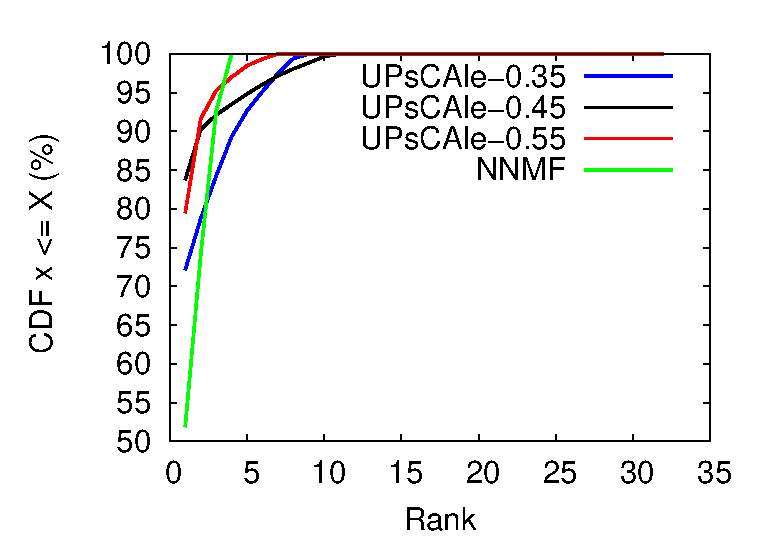
\epsfig{file=figures/topicDistributionAgnews.eps,width=1.53in,height=1.13in}} \quad
% \subfigure[Observatory]{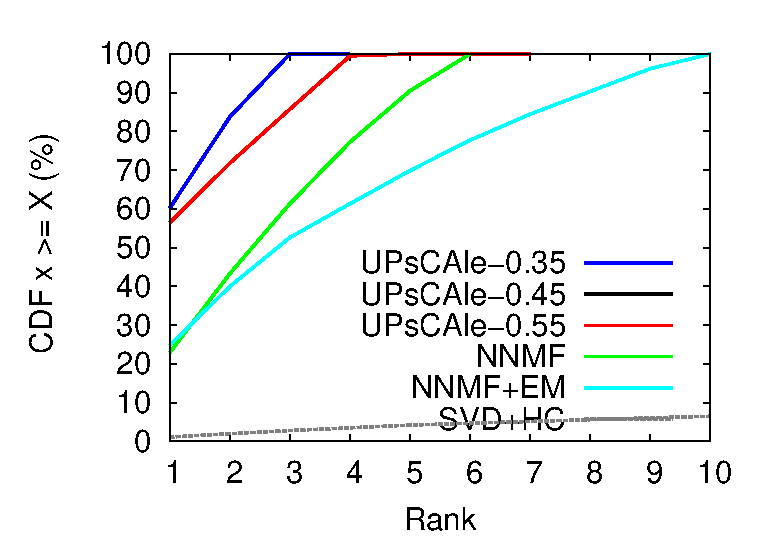
\epsfig{file=figures/topicDistributionObservatory.eps, width=1.53in,height=1.13in}}
% \subfigure[AgNews]{\epsfig{file=figures/numTopicsPerDocAgNews.eps, height=1.53in,width=1.13in,angle=-90}}
% \subfigure[Observatory]{\epsfig{file=figures/numTopicsPerDocObservatory.eps, height=1.53in,width=1.13in,angle=-90}}
% \caption{Topics most frequently assigned to documents (a) and (b), and the average number of topics assigned per document (c) and (d) for both agNews and Observatory}
% \label{fig:histograms}
% \end{figure*}


Apart from the two aforementioned metrics, we also calculate the precision and recall of the topics. The way precision and recall are calculated depend on how the documents are mapped to topics found and how topics are mapped to the known classes. Recall that a post can be associated with zero, one or more topics. Similarly, a topic can be mapped to one or more classes.
Hence, when precision and recall are calculated, they consider only the documents that belong to at least one topic. For this reason, we refer to the precision and recall metrics as an ``estimated" precision and recall, or e-precision and e-recall. 

The evaluation measures showed here were calculated under four scenarios. The first, named 1-1\_1-1, maps one document to one topic, and one topic to one class. This is the most restrictive metric, which associates the document with the most probable topic and the topic with the most frequent class among the documents in that topic. The second, 1-1\_N-1, maps one document to one topic but $n$ topics to one class. In this case, classes may refer to more than one topic. The third measure allows one document to be mapped to more than one topic, and again more than one topic may be associated with a single class (1-N\_N-1). Finally, the less restrictive metric is 1-N\_N-N, which maps one document to $n$ topics, and these $n$ topics with $n$ classes, characterizing a multi-label class problem.
For the first three cases, e-precision and e-recall are calculated using the tradition precision formula \cite{witten:2005}. For the fourth case, a multi-label version of these metrics is used \cite{tsoumakas2007multi}. 

In cases where the number of topics found is greater than the number of actual classes, depending on which type of topic-class mapping is being used, only the topics with the highest number of documents are mapped to the real classes, and this is reflected in the recall of the methods. 
\begin{figure}[!t]
\centering
	\subfigure{
		\begin{minipage}[c]{.05\textwidth}
			\vspace{-0.6cm}
			\hspace{-0.6cm}
			\centering
			\begin{sideways}
				\begin{scriptsize} \textbf{Avg number of topics} \end{scriptsize}
			\end{sideways}
		\end{minipage}
		\begin{minipage}[c]{.43\textwidth}
			\vspace{-0.4cm}
			\hspace{-0.5cm}
			\centering
\begin{minipage}[b]{0.45\linewidth}
			\subfigure{\epsfig{file=figures/numTopicsPerDocObservatory.eps, height=1.73in,width=1.10in,angle=-90}}
\end{minipage}
\hfill
\begin{minipage}[b]{0.45\linewidth}
			\subfigure{\epsfig{file=figures/numTopicsPerDocAgNews.eps, height=1.73in,width=1.10in,angle=-90}}
\end{minipage}

		\end{minipage}
	}
%%	\vspace{-0.3cm}
	\caption{Topics most frequently assigned to documents %(a) and (b), and the average number of topics assigned per document (c) and (d) 
	for Observatory and agNews}
	\label{fig:histograms}
\end{figure}

Considering these metrics, \method is compared with three other semantic topic identification techniques. The first, NMF, corresponds to the first part of \method and does not perform any merging of topics after finding the latent factors. The second applies a hierarchical average-linkage clustering algorithm to the topics extracted using Singular Value Decomposition (SVD), as done in \cite{kuhn2007semantic}. A version of Matlab's hierarchical clustering algorithm was used. Finally, the third method applies the expectation-maximization algorithm %(Weka version \cite{witten:2005}) 
to the topics created by NMF to merge topics. In this case, instead of using the $PCA$ to find the number of latent factors needed for a given representation, we use a predefined number of latent factors defined by the formula given in \cite{kuhn2007semantic}. A second version of this baseline, replacing NMF by SVD was also tested, and the results were statistically worst than those reported here.
For all baselines, the mapping between topics and classes follows the same principles as for UPsCALe. NMF runs for 100 iterations in all
cases.


\subsubsection{Experimental Results}

For the two labelled datasets, AgNews and Observatory, we report a subset of tests with different levels of topics representativeness (35\%, 45\% and 55\%) and $\alpha$ (0.3 and 0.5). % and 0.7.) 
As the topic-document mapping plays an important role during evaluation, Figure~\ref{fig:histograms} shows %the cumulative distribution function (CDF) for the most frequently assigned topics. %, and 
the number of documents to which 1, 2 and 3 topics were assigned. The analysis shows that no more than 3 topics were assigned to any document in both datasets. As data representativeness increases and reaches 55\% the number of documents assigned to more than two topics increases, but all baselines considered are assigned only one topic per document. Note that the values for SVD-HC and NMF+EM are not shown for agNews because they present a prohibitive computational time. \looseness=-1


Table~\ref{tbl:topics} shows the average results obtained over 10 runs of the methods. Results are compared using a two-tailed t-test with significance level 0.95. The second column shows the method considered: UPsCAle, SVD+HC, NMF+EM and NMF. For the latter, the number of latent factors to be found ($k$) is set as the number of known topics. In the case of UPsCAle, it is followed by the data representativity required (given as a parameter to PCA, which returns $k$). When the value of representativeness is missing, $k$ is set to $(m \times n)^2$ \cite{kuhn2007semantic}. The next two columns, under the name \# Topics, show the number of topics returned by PCA ($k$) followed by the final number of topics, obtained after running the merging phase of UPsCAle ($k'$). Note that, for AgNews, although the initial number of given topics was 12, this value decreased to 5 after the document-topic mapping, as documents belonging to 7 different small classes did not belong to any topics. The next column, Docs with Topics, shows the fraction of documents which were assigned to at least one topic. We emphasize that the metrics of e-precision and e-recall for the four situation previously described provided in the next columns were calculated over these documents.

\begin{figure}[!tb]
 \centering
 \subfigure[Observatory]{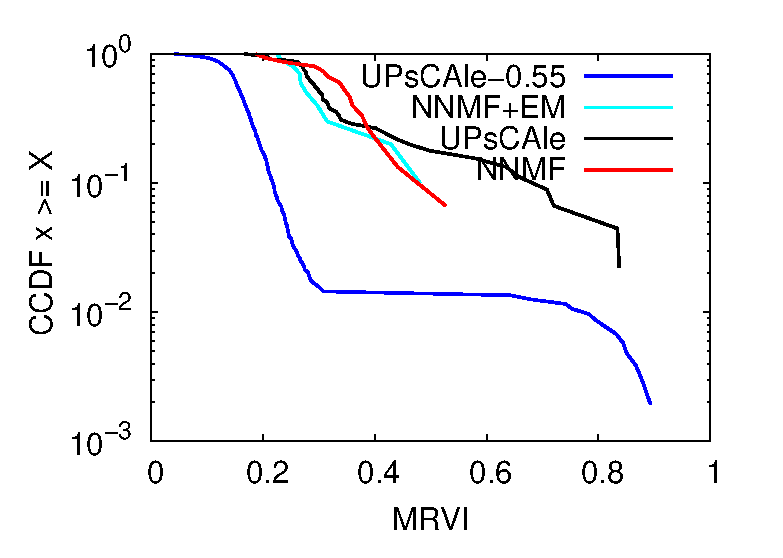
\epsfig{file=figures/topicsFragmentationObservatory.eps,height=1.4in,width=1.5in}}
% \subfigure[Observatory]{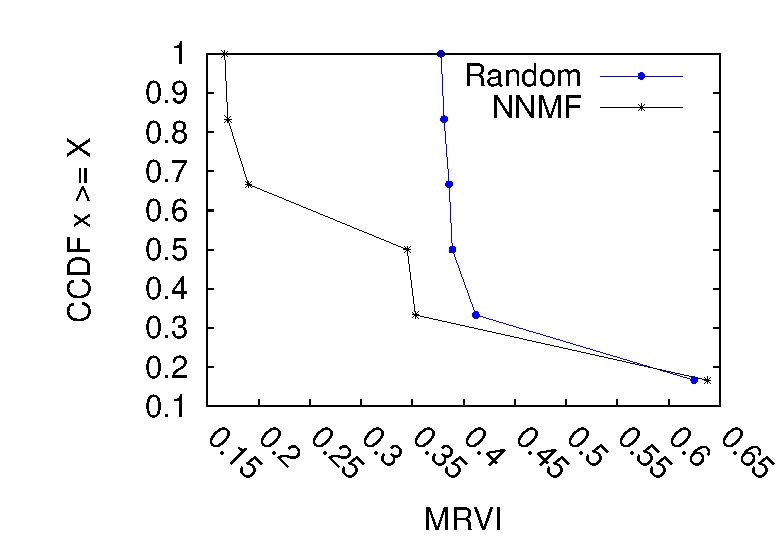
\epsfig{file=figures/fragmentation-Observatory-KT.eps, width=1.8in,height=1.45in}}
% \subfigure[Observatory]{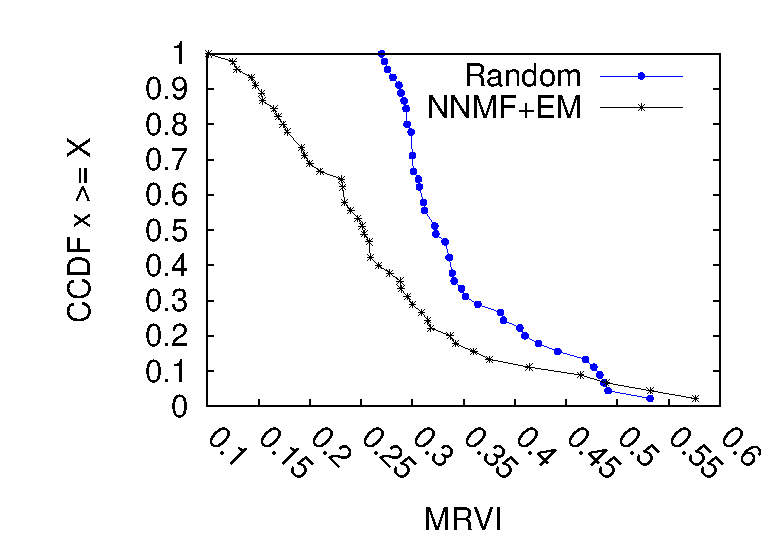
\epsfig{file=figures/fragmentation-Observatory-CL.eps, width=1.8in,height=1.45in}}
% \subfigure[AgNews]{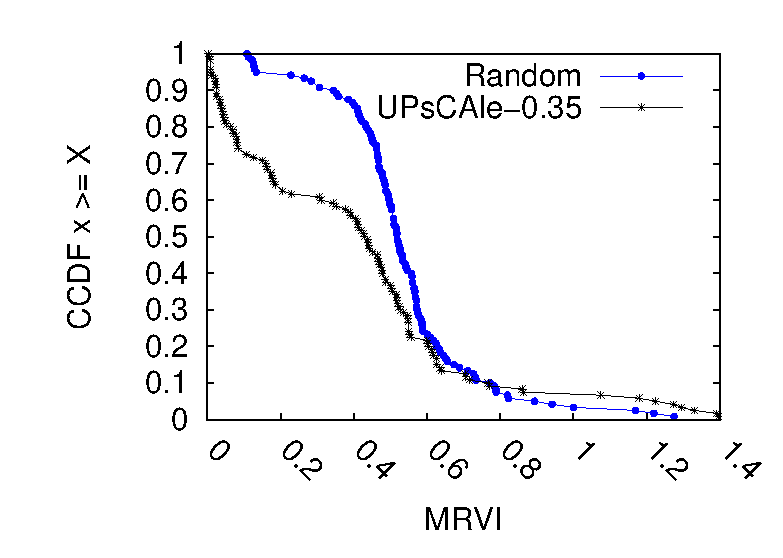
\epsfig{file=figures/fragmentation-agnews-upscale.eps,width=1.8in,height=1.45in}} %0.35
 \subfigure[AgNews]{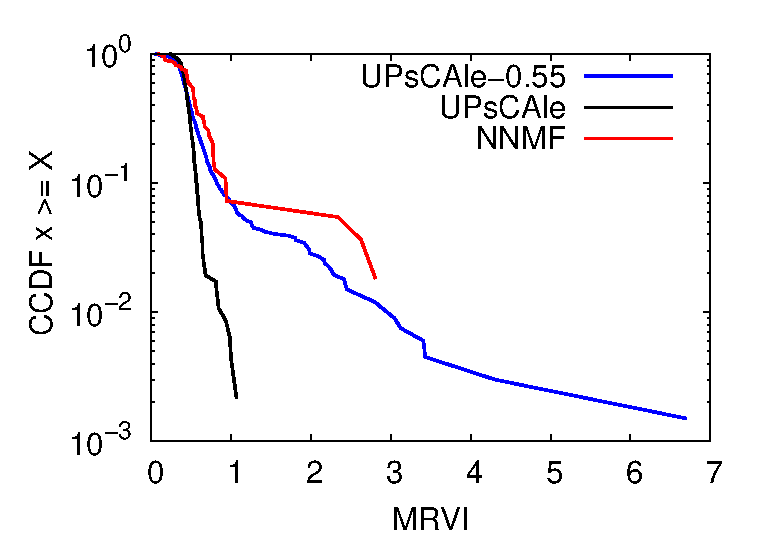
\epsfig{file=figures/topicsFragmentationAgNews.eps,height=1.4in,width=1.5in}}
 \caption{Distribution of $MRVI$ among all pairs of topics}
 \label{fig:mrvi}
 \end{figure}

In general, we observe that the higher the representativeness, the higher the number of covered examples, as more topics cover more documents. Similarly, the higher the value of cohesion, the higher the number of final topics $k'$, as the topics become more fragmented to be more cohesive. The differences between $k$ and $k'$ show that the merging process proposed significantly reduces the number of topics found.
In average, the proposed method performed 19 iterations for Observatory and 29 to AgNews.


Now looking at the Observatory dataset. 
The number of documents assigned to at least one topic varied from 88 to 99\% according to different representativeness.
When the number of topics was previously set, this number decreased to 40\%. 
In order to analyse precision and recall, we select one of the results and compare it against the others using the t-test. The results compared are highlighted in gray, and the symbol \textcolor[rgb]{00,0.45,0.10}{$\blacktriangle$} in a cell indicates its result is better than the highlighted, \textcolor[rgb] {0.7,00,00}{$\blacktriangledown$} indicates it is worse and \textcolor[rgb]{0.7,0.7,0.0}{$\bullet$} that there is no statistical evidence to state any difference.


%\newcommand{\green}{\cellcolor{green}}
%\newcommand{\red}{\cellcolor{red}}
%\newcommand{\norm}{\cellcolor{blue}}

\newcommand{\green}{\textcolor[rgb]{00,0.45,0.10}{$\blacktriangle$}}
\newcommand{\red}{\textcolor[rgb] {0.7,00,00}{$\blacktriangledown$}}
\newcommand{\norm}{\textcolor[rgb]{0.7,0.7,0.0}{$\bullet$}}




\begin{sidewaystable}
%\begin{table*}
%\begin{scriptsize}
\caption{ Results obtained for Observatory and AgNews. Documents with topics represent the number of documents assigned to at least one topic. The metrics of precision and recall are calculated under these documents. The four cenarious presented considering different mapping of Doc\_Topic\_Topic\_Class. \\}
\label{tbl:topics}



\begin{tabular}{|c||c|c|c|c||c|c|c|c|c|c|c|c|c|}
\hline
Cohesion&\multirow{2}{*}{Method}&\multicolumn{2}{c|}{\#Topics}&Docs &\multirow{2}{*}{Purity}&\multicolumn{2}{c|}{1-1\_1-1} &\multicolumn{2}{c|}{1-1\_N-1} &\multicolumn{2}{c|}{1-N\_N-1} &\multicolumn{2}{c|}{1-N\_N-N}\\ \cline{3-4}\cline{7-14}
         	($\alpha$) &          &     k    &      k'       & with Topics    &  & e-prec.   & e-recall          & e-prec.   & e-recall          & e-prec.   & e-recall          & e-prec.   & e-recall          
\\ \hline \hline

 \multicolumn{14}{|c|}{\textbf{Observatory}} 
\\ \hline \hline

\multirow{4}{*}{0.30} 
  & UPsCAle-0.35 & 115& 15.6 & \red 0.883 & \red 0.641 & \red 0.574 & \green 0.380 & \norm  0.477 & \green 0.435 & \norm  0.437 & \green 0.466 & \norm 0.789 & \green 0.884
\\ 
 & UPsCAle-0.45 & 171& 23.3 & \red 0.968 & \red 0.678 & \red 0.579 & \green 0.280 & \norm 0.461 & \green 0.358 & \norm 0.422 & \green 0.395 & \red 0.757 & \red 0.863
\\ \index{•}
 & UPsCAle-0.55 & 242& 31.3 & \norm 0.995 & \red 0.685 & \red 0.554 & \green 0.217 & \norm 0.451 & \green 0.304 & \norm 0.406 & \green 0.342 & \red 0.753 & \norm 0.873
\\
& UPsCAle & 25 & 5.9 & \red 0.391 & \green 0.825 & \red 0.520 & \green 0.429 & \norm  0.494 & \green 0.450 & \green 0.476 & \green 0.455 & \green 0.852 & \norm 0.868
\\ \hline{}

\multirow{4}{*}{0.50} 
 & UPsCAle-0.35 & 115& 25.1   & \red 0.885 & \red 0.696 & \red 0.582 & \green 0.283  & \green 0.473 & \green 0.364  & \norm 0.434 & \green 0.390  & \norm 0.769 & \red 0.855  
\\
 & UPsCAle-0.45 & 171 & 32.9  & \red 0.963 & \red 0.698 & \norm  0.631 & \green 0.244  & \norm 0.461 & \green 0.326  & \norm 0.413 & \green 0.363  & \red 0.761 & \red 0.864  
\\ 
 & \multicolumn{1}{| >{\cellcolor[gray]{0.85}}c|}{UPsCAle-0.55} & \multicolumn{1}{| >{\cellcolor[gray]{0.85}}c|}{242}& 
 \multicolumn{1}{| >{\cellcolor[gray]{0.85}}c|}{43.9}    & \multicolumn{1}{| >{\cellcolor[gray]{0.85}}c|}{0.995} & 
 \multicolumn{1}{| >{\cellcolor[gray]{0.85}}c|}{0.745} &  \multicolumn{1}{| >{\cellcolor[gray]{0.85}}c|}{0.657} & 
 \multicolumn{1}{| >{\cellcolor[gray]{0.85}}c|}{0.175}  & \multicolumn{1}{| >{\cellcolor[gray]{0.85}}c|}{0.438} & 
 \multicolumn{1}{| >{\cellcolor[gray]{0.85}}c|}{0.247}  & \multicolumn{1}{| >{\cellcolor[gray]{0.85}}c|}{0.404} & 
 \multicolumn{1}{| >{\cellcolor[gray]{0.85}}c|}{0.271}  & \multicolumn{1}{| >{\cellcolor[gray]{0.85}}c|}{0.773} & 
 \multicolumn{1}{| >{\cellcolor[gray]{0.85}}c|}{0.873}
 \\
 & UPsCAle & 25 & 9.7    & \red 0.395 & \norm 0.747 & \norm 0.631 & \green 0.442  & \green 0.566 & \green 0.508  & \green 0.552 & \green 0.516 & \green 0.859 & \norm 0.883

\\ \hline	


%\multirow{4}{*}{0.70} 
% & UPsCAle-0.35 & 115& 29.9 & \red 0.889 & \red 0.682 & \norm 0.655 & \green 0.288 & \green 0.513 & \green 0.398 & \green 0.466 & \green 0.430 & \norm 0.768 & \red 0.855
%\\ 
% & UPsCAle-0.45 & 171& 38.1 & \red 0.967 & \red 0.699 & \norm 0.622 & \green 0.218 & \norm 0.448 & \green 0.315 & \norm 0.412 & \green 0.348 & \norm 0.775 & \norm 0.873
%\\ 
% & UPsCAle-0.55 & 242& 43.7 & \norm 0.995 & \norm 0.745 & \norm 0.623 & \norm 0.179 & \norm 0.458 & \green 0.261 & \norm 0.399 & \green 0.284 & \green 0.810 & \green 0.907 
%\\
%& UPsCAle  & 25 & 17.2 & \red 0.399 & \red 0.602 & \norm  0.732 & \red 0.405 & \green 0.653 & \green 0.645 & \green 0.642 & \green 0.657 & \green 0.830 &  0.865
%\\ \hline 


\multirow{4}{*}{-} 
 & SVD+HC & - &2,333 & \green 0.999 & \red 0.354 & \green 0.898 & \red 0.024 & \green 0.776 & \green 0.775 & \green 0.776 & \green 0.775 & \green 0.956 & \green 0.956
\\ 
 & NMF+EM & 25 & 12.7 & \red 0.925 & \red 0.540 & \red 0.435 & \green 0.289 & \norm 0.390 & \green 0.415 & \norm 0.390 & \green 0.415 & \green 0.812 & \red 0.812
\\ 
 & NMF & 6 & 6.0 & \red 0.111 & \green 0.780 & \norm 0.670 & \green 0.629 & \green 0.671 & \green 0.699 & \green 0.669 & \green 0.700 & \green 0.921 & \green 0.923  
\\ \hline	


\hline

\multicolumn{14}{|c|}{\textbf{AgNews}} 
\\ \hline \hline
 
 \multirow{3}{*}{0.30} 
  & UPsCAle-0.35 & 59&  13.9 & \red 0.011 & \red 0.559 & \red 0.181 & \green 0.191 & \red 0.200 & \green 0.204 & \norm 0.200 & \green 0.204 & \norm 0.763 & \green 0.836
\\ 
 & UPsCAle-0.45 & 103& 19.4 & \red 0.085 & \red 0.694 & \red 0.242 & \green 0.166 & \norm 0.206 & \green 0.181 & \norm 0.207 & \green 0.186 & \green 0.781 & \green 0.806
\\ 
 & UPsCAle-0.55 & 163& 31.9 & \norm 0.359 & \norm 0.803 & \norm 0.246 & \norm 0.125 &  \norm 0.212 & \norm 0.137 & \norm 0.197 & \norm 0.140 & \norm 0.762 & \norm 0.797
\\
& UPsCAle        & 154 & 29.5 & \norm 0.283 & \norm 0.796 & \red 0.242 & \green 0.143 & \norm 0.212 & \norm 0.154 & \norm 0.189 & \norm 0.154 & \green 0.765 & \green 0.796 
\\ \hline{}


\multirow{3}{*}{0.50} 
 & UPsCAle-0.35 & 59& 16.5   & \red 0.011 & \red 0.557 &  \red 0.229 & \green 0.219  & \norm 0.227 & \green 0.238  & \norm 0.231 & \green 0.239  & \green 0.784 & \green 0.855
\\
 & UPsCAle-0.45 & 103 &  24.1  & \red 0.090 & \red 0.693 & \norm  0.309 & \green 0.183  & \norm 0.256 & \green 0.202  & \norm 0.248 & \green 0.207  & \green 0.776 & \green 0.802
\\ 
 

 & \multicolumn{1}{| >{\cellcolor[gray]{0.85}}c|}{UPsCAle-0.55} & \multicolumn{1}{| >{\cellcolor[gray]{0.85}}c|}{163}& 
 \multicolumn{1}{| >{\cellcolor[gray]{0.85}}c|}{34.4}    & \multicolumn{1}{| >{\cellcolor[gray]{0.85}}c|}{0.360} & 
 \multicolumn{1}{| >{\cellcolor[gray]{0.85}}c|}{0.810} &  \multicolumn{1}{| >{\cellcolor[gray]{0.85}}c|}{0.292} & 
 \multicolumn{1}{| >{\cellcolor[gray]{0.85}}c|}{0.117}  & \multicolumn{1}{| >{\cellcolor[gray]{0.85}}c|}{0.252} & 
 \multicolumn{1}{| >{\cellcolor[gray]{0.85}}c|}{0.132}  & \multicolumn{1}{| >{\cellcolor[gray]{0.85}}c|}{0.235} & 
 \multicolumn{1}{| >{\cellcolor[gray]{0.85}}c|}{0.137}  & \multicolumn{1}{| >{\cellcolor[gray]{0.85}}c|}{0.751} & 
 \multicolumn{1}{| >{\cellcolor[gray]{0.85}}c|}{0.783}
 \\
 
 
 
 
 & UPsCAle & 154 &   31.9   & \norm 0.283 & \red 0.787 & \norm 0.304 & \green 0.139  & \norm 0.245 & \green 0.157 & \norm 0.228 & \green 0.165  & \green 0.770 & \green 0.799 
\\ \hline

%\multirow{3}{*}{0.70} 
% & UPsCAle-0.35 & 59& 38.3 & \red 0.011 & \red 0.335 & \norm 0.413 & \green 0.328 & \green 0.388 & \green 0.394 & \green 0.382 & \green 0.387 & \green 0.790 & \green 0.882
%\\ 
% & UPsCAle-0.45 & 103& 56.7 & \red 0.085 & \red 0.468 & \green 0.471 & \green 0.235 & \green 0.419 & \green 0.354 & \green 0.419 & \green 0.358 & \green 0.777 & \green 0.819
%\\ 
% & UPsCAle-0.55 & 163& 42.1 & \norm 0.341 & \red 0.741 & \green 0.382 & \green 0.180 & \green 0.321 & \green 0.206 & \green 0.299 & \green 0.215 & \green 0.775 & \green 0.815
%\\
%& UPsCAle       & 154 & 39.1 & \norm 0.283 & \red 0.743 & \green 0.387 & \green 0.194 & \green 0.316 & \green 0.217 & \green 0.305 & \green 0.225 & \green 0.787 & \green  0.822
%\\ \hline
- & NMF & - & 11 & - & - & - & - & - & - & - & - & - & - 
\\ \hline

\end{tabular}



%\end{scriptsize}
%\end{table*}

\end{sidewaystable}












Analysing the precision and recall, \method with $\alpha=0.5$ and 0.55 representativeness was chosen as a reference, as it will cover more documents and set an equal trade-off for cohesion and uniqueness. Comparing these results with the other using $\alpha=0.3$, for all e-precisions except the most restrictive, the results found are better than the reference. Looking at the baselines, the results of SVD+HC seem far better than those obtained by UPsCAle. However, note that SVD+HC found 2,333 clusters. In the evaluation process, as only six clusters were mapped to the real classes in the 1-1\_1-1 evaluation, the recall is around 2\%, explaining the high precision. NMF also presented a much higher e-precision and e-recall than UPsCAle, but the column ``Docs with Topics" shows that only 11\% of documents were assigned to at least one topic in this case. NMF+EM is the strongest competitor, but given its final number of topics, the fairest comparison is to compare it with UPsaAle-0.35 with $\alpha=0.3$. The latter covers 4\% less documents, but presents higher purity and both e-precision and recall for all mapping, except for the less restrictive precision. Hence, tuning $\alpha$ and the representativeness, we can obtain better results than the current methods more efficiently, as discussed below.  
The much lower purity of NMF+EM might be due to the final number of topics. %However, it corroborates the main criticism against using the number of latent factors defined by \cite{kuhn2007semantic}, which usually requires a small number of latent factors which will usually returned mixed semantic topics.


With respect to agNews, we observe a completely different situation. The cost of the baselines was prohibitive, and when 11 was given to NMF as the number of latent factors to be found (i.e. the number of known-topics), only 57 documents (out of 878,705) were assigned to topics. The values of assignment for \method are also low, reaching 36\% with the highest value of representativeness and 34 topics in average.

The last metric calculated over the labelled datasets, fragmentation, is showed in Figure \ref{fig:histograms}. The histograms for the two datasets are completely different (recall that the lower the MRVI, the better). For Observatory, the graph shows that \method 0.55 is superior, i.e., the topics found overlap less. For agNews, \method using the predefined number of topics is superior, but this is due to the size of the topics (clusters) generated. As they are smaller, they tend to overlap less, and hence MRVI is better. 

\begin{figure*}[!tb]
 \centering
\subfigure[]{
\includegraphics[width=1.6in,height=1.35in]{figures/cloudTags/top1-elections.png}}
\subfigure[]{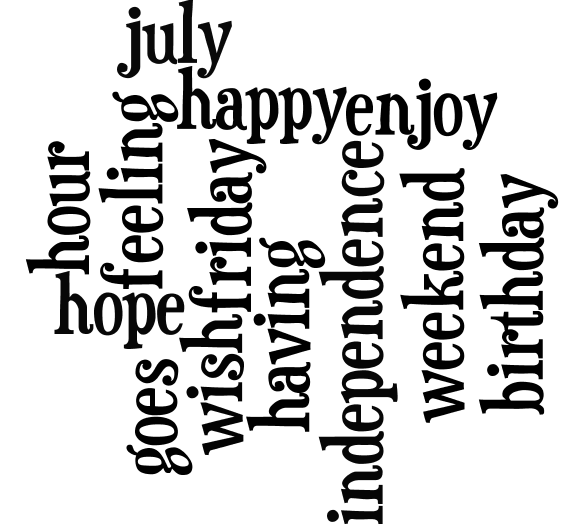
\includegraphics[width=1.6in,height=1.35in]{figures/cloudTags/top2-elections.png}} 
 \subfigure[]{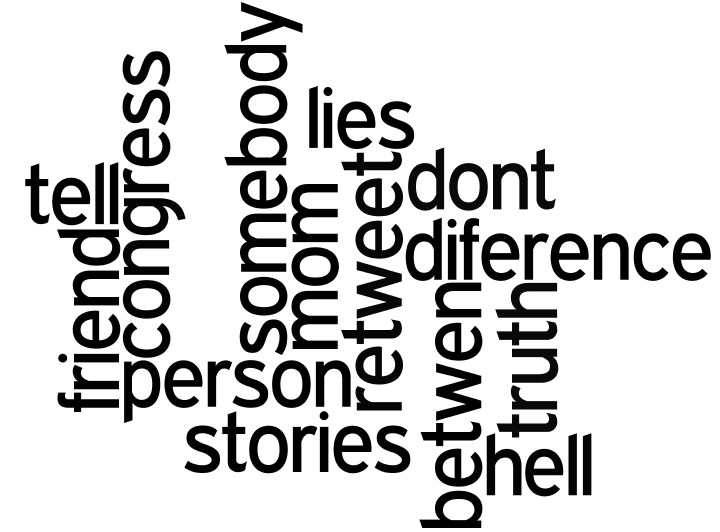
\includegraphics[width=1.6in,height=1.35in]{figures/cloudTags/top3-elections.png}}
 \subfigure[]{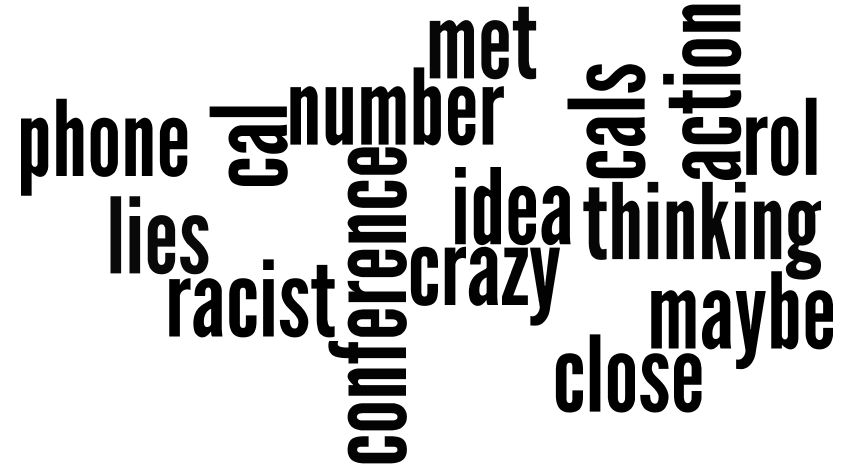
\includegraphics[width=1.6in,height=1.35in]{figures/cloudTags/top6-elections.png}} 
 \caption{Main topics discussed by Obama's followers: Independence Day, Democrats Convention in Sep. 2012 and gay marriage, Congress, and Call for an Ant-Racist Action.}
 \label{fig:election}
  \end{figure*}

\begin{table}[t]
\center
\begin{scriptsize}
\caption{Results obtained by UPsCAle considering Obama's followers in Twitter}\label{tbl:unlabeled}
\begin{tabular}{|l|l|l|l|l|}
\hline
 \multicolumn{5}{|c|}{Obama's Followers}  \\  \hline 
 \multirow{5}{*}{$\alpha$= 0.5} &\multirow{2}{*}{Repres.} & \multicolumn{2}{c|}{\#Topics} & \multirow{2}{*}{Purity}  \\ \cline{3-4}
 & & k & k' & \\ \cline{2-5}
 &0.35 & 94& 40.5 & 0.608 \\ %\cline{2-5}
 &0.45 & 141 & 43.75 & 0.613 \\ %\cline{2-5}
 &0.55 & 204 & 57.67 & 0.629 \\ \hline
%\multirow{3}{*}{FIAT} & \multirow{3}{*}{Framework} & 0,35 & 26 & 0.161 \\ \cline{3-5}
%&  & 0,45 & 47 & 0.144 \\ \cline{3-5}
%&  & 0,55 & 30 & 0.127 \\ \cline{3-5}
%\multirow{3}{*}{LouisVuitton} & \multirow{3}{*}{Framework} & 0,35 & 30 & 0.336 \\ %\cline{3-5}
%&  & 0,45 & 42 & 0.295 \\ \cline{3-5}
%&  & 0,55 & 61 & 0.153 \\ \hline
\end{tabular}
\end{scriptsize}
\end{table}

% \begin{table}
% \begin{tabular}{|l|l|l|l|l|}
% \hline
% Database & Repr & PCA & Clusters & Purity  \\ \hline
% \multirow{3}{*}{Election} & 0,35 & 94&34 & 0.617  --  0.535 \\ \cline{3-5}
% &  0,45 & 141 & 47 & 0.621  --  0.532 \\ \cline{3-5}
% &  0,55 & 204 & 52 & 0.652  --  0.552 \\ \hline
% %\multirow{3}{*}{FIAT} & \multirow{3}{*}{Framework} & 0,35 & 26 & 0.691  --  0.595 \\ \cline{3-5}
% %&  & 0,45 & 47 & 0.659  --  0.576 \\ \cline{3-5}
% %&  & 0,55 & 30 & 0.763  --  0.677 \\ \cline{3-5}
% %\multirow{3}{*}{LouisVuitton} & \multirow{3}{*}{Framework} & 0,35 & 30 & 0.635  --  0.475 \\ %\cline{3-5}
% %&  & 0,45 & 42 & 0.614  --  0.474 \\ \cline{3-5}
% %&  & 0,55 & 61 & 0.660  --  0.572 \\ \hline
% \end{tabular}
% \end{table}
% 


%\begin{table*}
\caption{Textual Description for the top-15 semantic topics identified in datasets agNews and Observatory.}\label{tbl:topicDescriptions}
\centering
	\begin{tiny}
	\begin{tabular}{|p{5.0cm}|p{5.0cm}|}\hline
		\textbf{AgNews}  & \textbf{Observatory} \\ \hline \hline
		
		che, non, con, una, roma, nel, calcio, man, dei, win, season, night, film, country, states  &  love, doctor, improvements, glory, going, strong, hope, world, hospital, night, know, brother, father, body, fever \\ \hline
		fedflare, style, latest, ful, story, both, details, read, display, none, release, version, releases, bok  &  slow, city, forward, thing, cause, brazil, center, hadad, street, look, debate, city, marcelo, height, support \\ \hline
		space, international, nasa, launch, shutle, station, atlantis, mission, astronauts, discovery, crew, agency, cape, canaveral, weather  &  live, earn, gremio, flu, corinthians, time, final, palmeiras, atletico, lose, guarani, goal, bahia, galo, fluminesne \\ \hline
		today, prnewswire, joke, leading, expected, usa, early, leaders, ago, firstcal, solutions, corporation, nbc, event, blockquote  &  with, and, con, new, audi, nissan, dodge, toyota, car, celta, auto, leader, corsa, strada, can \\ \hline
		set, record, fire, sets, start, date, deadline, final, take, loks, expected, anounce, begin, aside  &  back, show, psdb, twiter, follow, internet, win, pair, tickets, asks, civic, close, wake, guys \\ \hline
		plans, cut, sel, build, anounce, europe, largest, move, buy, part, corp, plant, cuts, expand, production  &  car, leaves, uno, music, advertising, caught, listen, telo, michel, like, commercial, santana, luan, success, thanks \\ \hline
		way, page, articlebody, our, used, fol, change, social, want, paving, fast, very, find, going, around  &  vasco, week, video, national, gama, \#euteamovasco, passed, earth, volleyball, shopping, visiting, ministry, praise, sea \\ \hline
		big, east, smal, brother, ten, scren, midle, dig, bowl, made, play, conference, money, much, another  &  makes, mean, kind, bottling, things, like, believer, stopped, santistas, passes, christian, part, chico, eating, \#santos \\ \hline
		through, thousands, weather, snow, riped, spam, strets, rain, swept, tore, another, water, hundreds, across, extension  &  friend, levy, Fidelix, man, mustache, aerotrem, hemorragic, be, party, birthday, minister, nobody, niece, sad, soninha \\ \hline
		anounced, conference, anounces, agrement, leading, prnewswire, global, awards, june, anual, feb, nasdaq, corporation, prize, march  &  saw, bad, beautiful, care, class, pretty, easy, sweetheart, arrives, here, leave, worse, step, wtf, dps \\ \hline
		life, real, prison, long, virtual, family, live, batery, sentenced, half, mars, scientists, insurance, water, bok  &  speech, team, ole, heart, name, fan, imagine, desire, crazy \\ \hline
		stil, despite, long, even, while, missing, though, death, another, remains, much, yet, god, although, ago  &  know, wanted, result, exam, morning, exams, ese \\ \hline
		now, long, ago, available, then, again, once, until, months, going, realy, change, wgc, same, wel  &  sunday, saturday, friday, schedule, guys, next, be, porto-alegre, candidates, grace, coming, friends, flu, decision \\ \hline
		plan, public, sharon, part, safety, proposal, spectrum  &  globe, making, novel, want, record, radio, network, play, teams, minister \\ \hline
		media, reported, chinese, reports, player, beijing, television, times, newspaper, digital, content, comission  &  stay, rain, neymar, give, accept, ring, trapped, missing, elections, place up, start, eat, celso \\ \hline
% 		internet, users, acess, ogi, aol, broadband, net, computer, explorer, ban, chinese, fre, browser, providers, ican & & \\ \hline
% 		search, engine, results, desktop, users, aol, market, fast, local, information, msn, tol, enterprise, missing & & \\ \hline
% 		che, con, una, roma, dela, calcio, nel, dei, ala, dal, sono, gli, due, italia, dele & & \\ \hline
% 		option, issue & & \\ \hline
\end{tabular}
\end{tiny}


% \begin{minipage}[t]{0.35\linewidth}
% \begin{tiny}
% \begin{tabular}{|p{6cm}|}
% \hline
% \textbf{Obamas' Followers}  \\ \hline \hline
% year, ago, boy, milion, girl, election, bilion, woman, low, olds, past, katc, rest, aniversary, half\\ \hline
% thought, prety, loks, col, funy, idea, haha, wow\\ \hline
% litle, bit, girl, boy, sems, late, girls, kid\\ \hline
%  stop, making, dear, rest, neds, giving, voter, caling, sign, shop, web, shit, boy, thinking, ful\\ \hline
%  fun, making, loks, sounds, stuf, times, guys, wekend, sumer, play, music, fod, miss, glad, join\\ \hline
%  hey, girl, guys, folow, met, remember, crazy\\ \hline
%  yeah, hel, haha, prety, fuck, remember, bit, sems, gona, shit, stuf, kind, crazy, sounds, heard\\ \hline
%  money, buy, pay, making, spend, government, walker, save, raise, taxes, rich, politics, giving\\ \hline
% isn, problem, working, funy, person, runing, kind, question, issue, word, aren, anymore, shit, fredom, worth\\ \hline
%  lot, stuf, parking, sems, means, loks, shit, sounds, folks, coming, wow, kind, hear, agre, hel\\ \hline
%  big, deal, fan, government, brother, business, data, lie, smal, banks, oil, coming, dog, diference, gov\\ \hline
% hate, republicans, crime, gona, shit, gay, fucking, anti, fuck, haters, anger, lies, sems, stupid, side\\ \hline
%  nice, met, loks, guys, hear, haha, play, place, piece, pic, wekend, shot, person\\ \hline
% bad, breaking, idea, guys, economy, ass, prety, worse, wasn, season, person, luck, movie, problem, girls\\ \hline
% actualy, prety, funy, caled, kind, problem, hapened, thinking, haha, agre, idea, word, sems, wow, runing\\ \hline
%  put, place, end, neds, biden, face, fire, gona, head, line, dog, chains, joe, car, hands\\ \hline
%  geting, ready, started, married, finaly, excited\\ \hline
%  home, bring, stay, coming, swet, dog, lost, ofice, working, mom, sales, neds, kids, place, leave\\ \hline
%  made, laugh, mistake, decision, joke, remember, sense, china, clear, case, point, movie, finaly, choice, totaly\\ \hline
% start, neds, business, shit, gona, head, end, season, caled, place, wekend, fire, early, bok, tomorrow\\ \hline
% fre, market, download, stuf, fredom, buy, country, shiping, fod, sign, open, iphone, bok, riot, tickets\\ \hline
%  talk, hear, radio, politics, listen, shit, economy, political, ted, shows, listening, abt, issues\\ \hline
% doesn, mater, understand, sem, change, sound, exist, sense, count\\ \hline
%  didn, build, hear, realize, bush, hapen, glad, mention, guess, told, wouldn, wanted, notice, wasn, knew\\ \hline
% kep, coming, mind, open, truth, fight, eye, posted, teling, head, stuf, safe, voting\\ \hline
% guy, told, guys, kind, car, girl, funy, caled, heard, runing, face, pick, rich, gay, hel\\ \hline
% cal, phone, conference, rol, police, caled, number, close, racist, fire, action, cals, crazy, lies, wake\\ \hline
% awesome, loks, prety, guys, amazing, sounds, haha, met, totaly, stuf, dude, wow, congrats, gona, place\\ \hline
%  tel, truth, congress, lies, lie, friends, diference, betwen\\ \hline
% fel, makes, sense\\ \hline
%  things, change, hapen, diferent, worse, wrong, aren, important, miss, lots, favorite, buy, hear, learn, amazing\\ \hline
%  lok, loking, forward, seing, folow, wekend, tomorrow, makes, face, making, hair, eyes, loks, wow\\ \hline
%  los, con, son, por, del, para, usa, las, una, mas, pero, como, angeles, coming, esta\\ \hline
% updates, family, akin, war, state, schol, jobs, convention, rape, plan, morning, top, spech, twiter, part\\ \hline
% \end{tabular}
% \end{tiny}
% \end{minipage}
\end{table*}



% \begin{figure*}[!tb]
% \centering
% \subfigure[Football]{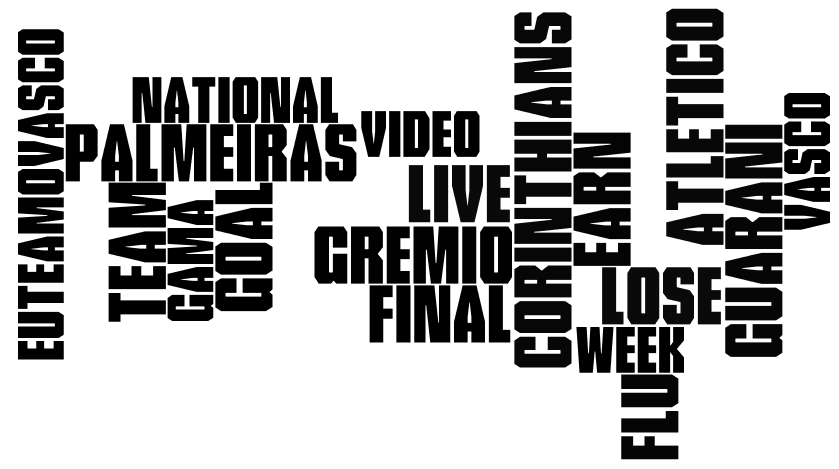
\includegraphics[width=1.5in,height=1.45in]{figures/cloudtags/football.png}}
% \subfigure[Cars]{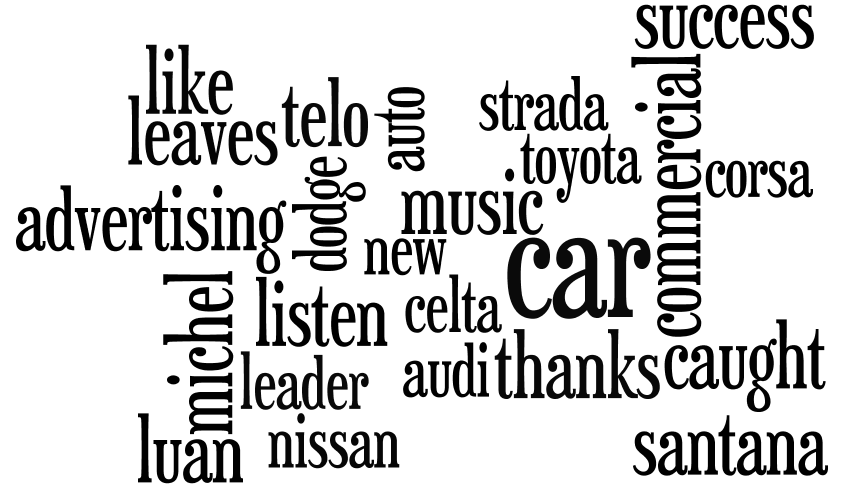
\includegraphics[width=1.5in,height=1.45in]{figures/cloudtags/car.png}}
% \subfigure[Dengue Fever]{
\includegraphics[width=1.5in,height=1.45in]{figures/cloudtags/dengue.png}}
% \subfigure[Politics]{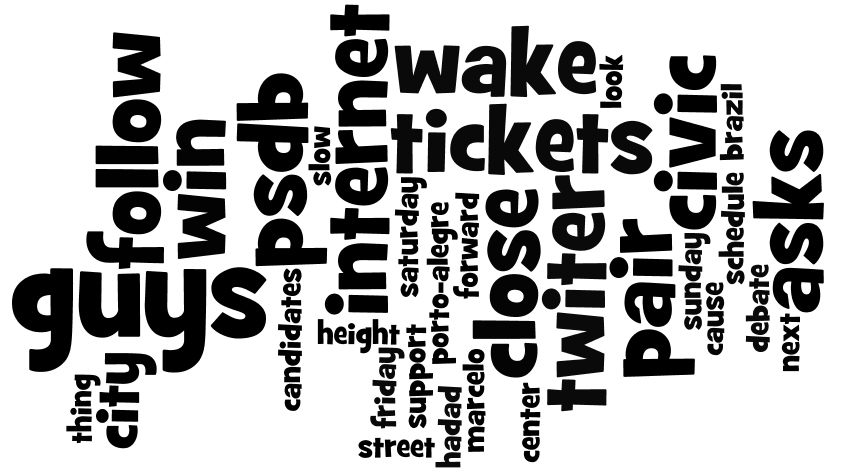
\includegraphics[width=1.5in,height=1.45in]{figures/cloudtags/politics.png}} 
% \caption{Main terms found in the top-4 topics in the Observatory dataset}
% \label{fig:topics}
% \end{figure*}


%However, the best way to evaluate the job being done by the method is to look at the topics generated. Table~\ref{tbl:topicDescriptions} shows the top-15 topics for Observatory and agNews. \gi{comparar com as classes do agnews}

From the results previously discussed, we can conclude that \method presents solutions statistically better than those obtained by the baselines when the value of $\alpha$ is tuned accordingly. The semantics of the topics is also good, but results are omitted here due to space restrictions, and presented in the case study in the next section. More importantly, the proposed framework was conceived to scale to bigger datasets. This is its main advantage over the baselines that aim to reduce the number of topics. While EM is linear in the number of documents $N$, the proposed algorithm depends on the number of latent factors $k$ used to describe $N$ and in the diameter $d$ of the graph. Algorithm 1 has time complexity O($(k-1) \times d \times k^3$), where k-1 is the maximum number of 
iterations.

%\begin{figure}[!th]
%\center
%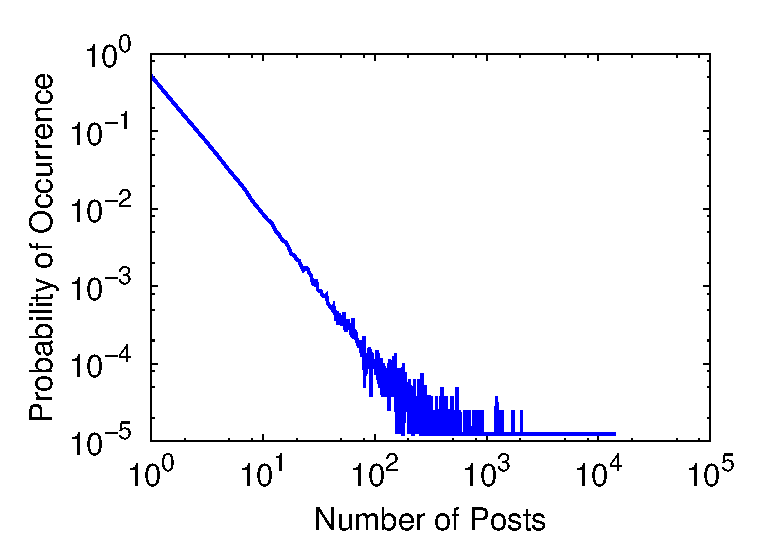
\epsfig{file=figures/postFrequencyElection.eps,width=2in,height=1.5in}
%\caption{Post frequency per user for Election}
%\label{fig:election}
%\end{figure}

\subsection{Obama's Followers: A Case Study}

This section presents a case study for characterizing a specific group of Twitter users: Obama's followers. The dataset was collected from July to September 2012. %Figure~\ref{fig:election} shows the post frequency per user in the period. 

Recall that, for this dataset, we do not know the discussed topics. Hence, we evaluated the quality of the generated clusters by using an adaptation of the purity metric defined in Eq. 5. Instead of considering the purity of the clusters with respect to the real class, we evaluate the purity of the terms across different groups, as done in \cite{kao2004mining} with entropy.
The results are shown in Table~\ref{tbl:unlabeled}, and for all three data representativeness used, the results of purity are very similar.

Here we perform a more detailed analysis of how topics are merged and how these merges improve user characterization with semantic topics. For this dataset, 33 iterations of the method were performed. Figure~\ref{fig:election} shows four of the top-ten topics most that characterize 80\% of the users.
The first topics, showed in Figure~\ref{fig:election} (a), characterizes 70.5\% of the users. The topic related to the selection criteria of the users, which was indirectly politics. Its main subject is the Democrats convention in September 2012, which decided to support gay marriage. Note the terms \textit{son} and \textit{dog} are not directly related to the topic, and were added during the merge of almost half of NMF output files. 
Analysing the topics in the earlier levels of the merge, we observe that all merges relate to politics. However, it is interesting to notice that the method actually produces a hierarchy of topics, which will generate single topics if the maximum number of iterations is performed. Correctly choosing where to stop in the hierarchy can give the user the topics at the semantic level he wants. Fine-tuning the stopping criteria is the next step.

The second topic which characterizes users (Figure~\ref{fig:election} (b)) is related to the $4^{th}$ of July. It actually shows terms referring to the independence and others referring to wishes of happy birthday or references to a happy and enjoyable weekend. Here \method merged 9 different topics related to best wishes in various events. The third topic is a merge of two topics referring to the congress and its bills. The fourth topic relates to calls for an anti-racist act. Note that the term \textit{phone}, related to call, was associated to this topic in the NMF output.


%\begin{table}
\caption{Textual Description for the top-10 semantic topics identified for Obama's followers.}\label{tbl:topicDescriptionsObama}
\centering
	\begin{tiny}
	\begin{tabular}{|p{7.8cm}|}\hline
		Top-10 NNMF Semantic Topics \\ \hline \hline
wek,shark,friday,past,fashion,tampa,times,monday,sunday,sumer,starts,busy,wekend,fotbal,ready\\
top,stories,daily,times,ten,\#lastfm,artists,tweted,york,botom,bcvisionweb,gun\\
political,power,ads,politics,history,parties,system\\
akin,tod,race,rep,senate,coments,\#mosen\\
party,tea,democratic,platform\\
election,voter,law,voting,fraud,recal,presidential,voters,wisconsin,early,betwen,important,court,ohio,choice\\
america,bank,comunist,muslim,awake,united,states,anti,bless,destroy,fredom,garbage,founders,stand,nation\\
wrong,place,side,agre,word,sems,fuck,prove,person,law,totaly,speled,policy,question,facts\\
suport,marriage,\#txsen,child,equality,public,conservative,apreciate,congress,proud,govt,act,platform,retwet,sign\\
guy,told,kind,girl,car,runing,funy,heard,pick,rich,hel,asked,smart,face,wanted\\\hline\hline

Top-10 Semantic Topics after 5 iterations of the merging algorithm \\ \hline \hline

put,place,biden,gona,face,chains,line,hands,joe,mouth,word,car,front,charge,pants\\
awesome,sounds,totaly,dude,congrats,gona,wekend,fucking,place,super,amazing,kind,met,movie,glad\\
wrong,place,side,agre,word,sems,fuck,prove,person,law,totaly,speled,policy,question,facts\\
hard,working,hit,worked,die,drive,understand,easy,play,hiting,times\\
political,power,ads,politics,history,parties,system\\
world,life,real,change,climate,pro,shit,estate,rest,center,mind,trade,place,living,record\\
guy,told,kind,girl,car,runing,funy,heard,pick,rich,hel,asked,smart,face,wanted\\
los,times,fun,coming,por,son,idea,del,para,con,las,una,mas,pero,como\\
twiter,stuf,read,post,twet,check,folow,blog,twets,funy,folowers,reading,acount,interesting,found\\
police,dead,facebok,updates,woman,city,election,neds,game,convention,ago,americans,gay,rape,spech\\\hline\hline

Top-10 Semantic Topics after 9 iterations of the merging algorithm \\ \hline \hline

wow,amazing,crazy,shit,beautiful,fox,guess,words\\
put,place,biden,gona,face,chains,line,hands,joe,mouth,word,car,front,charge,pants\\
awesome,sounds,totaly,dude,congrats,gona,wekend,fucking,place,super,amazing,kind,met,movie,glad\\
wrong,place,side,agre,word,sems,fuck,prove,person,law,totaly,speled,policy,question,facts\\
hard,class,midle,working,taxes,rich,hit,worked,die,drive,understand,easy,play,hiting,times\\
caled,place,heard,biden,joe,word,song,reason,told,racist,movie,chris,john,stupid,mom\\
guy,told,kind,girl,car,runing,funy,heard,pick,rich,hel,asked,smart,face,wanted\\
los,times,fun,coming,por,son,idea,del,para,con,las,una,mas,pero,como\\
twiter,stuf,read,post,twet,check,folow,blog,twets,funy,folowers,reading,acount,interesting,found\\
police,dead,facebok,updates,truth,woman,city,election,neds,political,game,convention,ago,americans,gay\\\hline\hline

Top-10 Semantic Topics after 12 iterations of the merging algorithm \\ \hline \hline

col,hot,stay,super,totaly,sumer,air,music,sounds,place,dude,dad,pic,kinda,west\\
story,raw,cover,amazing,ful,told,sad,short,tels,link,interesting,bain,write,breaking,teling\\
wow,amazing,crazy,shit,beautiful,fox,guess,words\\
put,place,biden,gona,face,chains,line,hands,joe,mouth,word,car,front,charge,pants\\
awesome,sounds,totaly,dude,congrats,gona,wekend,fucking,place,super,amazing,kind,met,movie,glad\\
wrong,place,side,agre,word,sems,fuck,prove,person,law,totaly,speled,policy,question,facts\\
friends,wekend,fox,share,met,word,words,close,dear,liberal,enemies,open,conservative,colege,stay\\
talking,points,politics,clint,eastwod,chair,shit,abt,empty,economy,biden,heads,issues,fuck,joe\\
los,times,fun,coming,por,son,idea,del,para,con,las,una,mas,pero,como\\
police,dead,facebok,updates,truth,woman,city,election,neds,political,game,convention,ago,americans,gay\\\hline
\end{tabular}
\end{tiny}
\end{table}








\section{Conclusions and Future Work}

In this paper we analysed how the semantic topics can be used to extract
general characteristics from the users. 
We propose UPsCAle, a framework that works in three phases: it
identifies semantic sub-topics of a user group using a traditional matrix
factorization method and then merges those sub-topics into more cohesive
and unique semantic topics. In a last phase, it maps the final set of semantic
topics to users profiles.

The proposed method was evaluated considering two labelled dataset and an
unlabelled one. The results show that, when compared to other state of the art
methods for topic identification, \method can find better results than the baselines if the the trade-off between cohesion and uniqueness is
properly set. Furthermore, the method scales well to very large datasets.

As future works, the stopping criteria of \method will be carefully studied. As it generates a hierarchy of topics, identifying the level of interest to be explore is important. The method will also be enhanced with the approach proposed in \cite{cheng:2013} to deal better with data sparsity. Finally, other user characteristics will be added to the current profile.

%However, the same can be done with more spcific features. \gi{blabla}

\section{Origins and General Discussion}

The previous sections are part of an article sent to the SIAM International Conference on Data Mining 2014. It was a collaborative work with two doctorate students, namely Tiago Cunha and Fernando Mourão. I have worked mostly in the first 7 steps of the framework (see figure \ref{frameworkFig}), implementing and discussing ideas and hypothesis with the team.

The objectives of POC 1 were successfully achieved, and I was able to exercise the acquired knowledge throughout my undergraduate course.
During the development of the framework, new problems and ideas for future work were found. The first, and most important, is that the matrix of $posts \times words$ is very sparse and this can be a problem for the NMF algorithm. Dealing with sparsity is the first goal for POC 2. We will investigate a similar approaches to the one proposed in \cite{cheng:2013}.

The second objective of POC 2 is to make UPsCAle an online method. Currently, it is considered an offline method since it uses static input data, e.g. data do not vary over time. As we want to integrate it with \textit{Observatório da Web} we need to learn how to deal with streams of tweets and news. 





\bibliographystyle{sbc}
\bibliography{references}

\end{document}

% End of ltexpprt.tex
%
